\documentclass{article}

% arXiv version: use neurips_2024 in nonblind, with-titlepage style
\usepackage[final]{neurips_2024}

\usepackage[utf8]{inputenc}
\usepackage[T1]{fontenc}
\usepackage{hyperref}
\usepackage{url}
\usepackage{booktabs}
\usepackage{amsfonts}
\usepackage{amsmath}
\usepackage{nicefrac}
\usepackage{microtype}
\usepackage{xcolor}
\usepackage{graphicx}
\usepackage{subcaption}
\usepackage{enumitem}
\usepackage{multirow}

\hypersetup{
  colorlinks=true,
  linkcolor=blue!50!black,
  citecolor=blue!50!black,
  urlcolor=blue!50!black,
}

\title{User as Engram: Internalizing Per-User Memory as Local Parametric Edits}

\author{%
	Bojie Li \\
	Pine AI
}

\begin{document}

\maketitle

\begin{abstract}
Personal memory in LLMs is two problems, not one: \emph{content}
(per-user facts) and \emph{meta-skill} (reasoning patterns that use
facts to answer questions). Per-user LoRA conflates them in one
substrate. We show this is wrong both empirically and
architecturally: per-user LoRA produces large, measurable
contamination on text unrelated to the user's facts (validation bpb
$\Delta {=} {+}1.56$ on Mini-Engram-d20, a 2.1$\times$ increase from
0.74 to 2.30, hurting indirect reasoning in 17/20 users), while
per-user Engram-row insertion produces \emph{exactly} zero
contamination by construction
($\Delta{=}{+}0.0001$, $\sim$15{,}000$\times$ smaller). The two
mechanisms behave as their architecture predicts.

This motivates a \textbf{layered architecture}: one shared LoRA holds
cross-user meta-skill (amortised over the population), and per-user
Engram-row overrides hold per-user content (local, 88\,KB/user).
At $n{=}20$ test users on Mini-Engram-d20, the layered design
\textbf{Pareto-dominates} every per-user single-substrate baseline:
100\% direct top-1 recall (matches per-user LoRA), 6.8$\times$ better
indirect reasoning than per-user LoRA (44\% vs 7\%
indirect-any), 4.0$\times$ less contamination ($\Delta$bpb +0.39
vs +1.56), and \emph{never} hurts indirect reasoning relative to the
no-adapter base (0/20 vs 17/20 for per-user LoRA). The cross-user
LoRA is amortised: storage per user is the Engram's 88\,KB, not
14.2\,MB. Combining \emph{per-user} LoRA with per-user Engram (the
naive composition) gives the worst of both: contamination remains
high and indirect reasoning still collapses.

Cross-model replication on four instruction-tuned bases (Qwen2.5-3B at
$n{=}30$; Llama-3.1-8B, Mistral-7B-v0.3, Qwen2.5-7B each at $n{=}20$)
shows the original "5/10 users worse than base" claim was small-sample
artifact: at scale, per-user LoRA helps indirect reasoning on every
instruction-tuned base ($\Delta$ ${=}{+}0.088$ to ${+}0.217$) with
only 0–20\% of users worse. The
\emph{architectural} contamination is unambiguous; the
\emph{user-visible} effect depends on whether the base is an
instruction-tuned LM (LoRA mostly fine) or a base LM (LoRA
destructive in 85\% of users). The layered design works robustly
across both.

We further measure RAG head-to-head against the layered design (F)
on the same probes and find a cross-over driven by KB size. At a toy
KB (34 facts/user), Qwen2.5-3B-Instruct + RAG-top-3 reaches 52\%
indirect\_any vs F's 44\% (at 0 context tokens). At realistic KB
sizes ($N\in\{100,200,300,500,1000\}$ facts/user via a 30-user
distractor pool), \texttt{all-MiniLM-L6-v2} top-3 recall collapses
from 62\% to 9\%, and Qwen-3B + RAG-top-3 drops to \textbf{30\%
indirect\_any}—\textbf{14\,pp below F}, which is invariant in
this axis because per-user Engram tables don't grow with population
size. \textbf{At $N\geq 100$, F (zero context, no retrieval) beats
both naive RAG on the same Engram backbone and Qwen-3B + RAG} on a
$\sim$2.5$\times$ larger instruction-tuned model. The trade-off is
decided by deployment scale, not by which substrate alone.

We release four Mini-Engram weights spanning 178\,M–1.22\,B
parameters (the first publicly available Engrams outside
DeepSeek-AI), all training code, and complete result JSONs.
A 50-line multi-tenant server reaches 232\,req/s on one GPU
with zero cross-user leak by construction.
\end{abstract}

\section{Introduction}
\label{sec:intro}

Modern transformer~\citep{vaswani2017transformer} LLMs serve
millions of users from a single backbone, but per-user
\emph{personal memory}—the system's knowledge of \emph{your}
doctor, \emph{your} preferences, \emph{your} calendar—remains an
open architectural problem. Three families address it: in-context
learning (ICL,~\citealt{brown2020gpt3,min2022rethinking}) prefixes
the facts; retrieval-augmented generation
(RAG,~\citealt{lewis2020rag,gao2023ragsurvey}) fetches them at
query time; and per-user adapters internalise them as weight
deltas. The third family has accumulated a long list of variants
on the same recipe—PRAG~\citep{su2024prag},
DyPRAG~\citep{tan2025dyprag},
DistilledPRAG~\citep{distilledprag2025},
OPPU~\citep{tan2024oppu}, HYDRA~\citep{zhuang2024hydra},
MemLoRA~\citep{memlora2025}, T2L~\citep{t2l2024}, and
PER-PCS~\citep{tan2024perpcs} all train a per-user rank-$\sim$64
LoRA~\citep{hu2022lora,houlsby2019adapters} on $Q/K/V/O$ + MLP via
NTP on an (observation, fact, QA) mixture, then apply it on top of
a frozen base. We call this canonical recipe \textbf{POLAR-class}
when it serves as the reference point.

\paragraph{The motivating finding.}
We replicate POLAR-class training (rank-64 NTP on
observation/fact/QA mixtures, 12 epochs $\times$ 200 samples,
20--30 synthetic users $\times$ 50 facts) across four
instruction-tuned bases and one base LM, and measure both the
\emph{architectural} contamination (val\_bpb $\Delta$ on text
unrelated to the user's facts) and the \emph{user-visible} effect
(indirect-reasoning recall on the user's own probes). The two
properties decouple:

\begin{itemize}[leftmargin=*,topsep=2pt,itemsep=1pt]
  \item Direct recall with adapter: \textbf{1.000} on every base.
  \item Architectural contamination is large and replicable:
        val\_bpb $\Delta {=} {+}1.56$ on Mini-Engram-d20 (a 2.1$\times$
        increase from 0.74 to 2.30 on held-out ClimbMix text—15{,}000$\times$
        more contamination than Engram-row insertion's $+0.0001$).
  \item User-visible effect depends on the base: per-user LoRA hurts
        indirect reasoning in 85\% of users on Mini-Engram-d20 (a base LM),
        but helps on every instruction-tuned base we tested
        (Qwen-3B $\Delta {=} {+}0.088$ at $n{=}30$, Llama-8B ${+}0.188$,
        Mistral-7B ${+}0.217$, Qwen-7B ${+}0.132$, each at $n{=}20$).
        Our earlier $n{=}10$ pilot on Qwen-3B-Instruct (5/10 users worse
        than base) was a high-variance small-sample artifact;
        at $n{=}30$ the worse-fraction drops to 20\% with Wilson 95\%
        CI $[0.10, 0.37]$, and on the other three instruction-tuned
        bases it is 0--5\%.
\end{itemize}

The architectural contamination is the load-bearing claim:
\emph{any} per-user edit that is unconditionally active will affect
all forwards, including those that have nothing to do with the user's
facts. The mechanism is structural: a LoRA delta on $Q/K/V/O$
in every layer enters every forward pass.

\paragraph{The architectural requirement.}
\textbf{Per-user edits must be local: they should fire only on
forwards whose token sequence matches the fact's trigger, and be
mathematically inert everywhere else.} POLAR-class LoRA fails this
test by construction. We propose \textbf{User as Engram}: per-user
fact storage as surgical writes to the hash-keyed embedding table
of an Engram-pretrained model~\citep{cheng2026engram}, whose
context-aware gated lookups fire only on suffix N-grams via
deterministic multiplicative-XOR hashing. Per user, we write one
fact-row per trigger N-gram into an \emph{override map} and apply
it per request. The local-edit property is not an asymptotic
approximation but a measurable invariant: on Mini-Engram-d12, a
UNEMBED\_P insertion at the last Engram layer perturbs the
residual stream by \emph{exactly} 0.000 at every non-trigger
position, through every subsequent attention+MLP layer
(Section~\ref{sec:locality}, Figure~\ref{fig:locality}).

\paragraph{Contributions.}
\begin{enumerate}[leftmargin=*,topsep=2pt,itemsep=1pt]
  \item \textbf{A measurable contamination gap with a base-dependent
        user-level effect} (Section~\ref{sec:negative}): per-user LoRA
        produces 15{,}000$\times$ more val\_bpb contamination than
        per-user Engram-row insertion on the same Mini-Engram-d20 base
        ($\Delta {+}1.56$ vs ${+}0.0001$, $n{=}20$). The user-visible
        effect on indirect reasoning is high-variance and base-dependent:
        85\% worse on a base LM (Mini-Engram-d20), 0--20\% worse across
        four instruction-tuned bases (Qwen-3B at $n{=}30$;
        Llama-8B, Mistral-7B, Qwen-7B each at $n{=}20$).
  \item \textbf{Public Mini-Engram weights} (Section~\ref{sec:repro})
        at four dense sizes spanning 178\,M to 1.22\,B total
        parameters (51.2\,M Engram-table shared across sizes),
        trained from scratch on ClimbMix on a single Blackwell GPU.
        To our knowledge the first publicly available Engrams
        outside DeepSeek-AI.
  \item \textbf{Three insertion strategies and Joint OPT}
        (Section~\ref{sec:method}). Joint OPT (sparse-row joint
        training) roughly doubles both top-1 (68\% vs.\ 36\%) and
        top-5 (96\% vs.\ 54\%) over per-fact independent OPT at
        100 facts/user, at identical storage (88\,KB).
  \item \textbf{Scaling experiments anchored on a category
        breakdown.} A $5{\times}3{\times}2$ capacity ablation pins
        the optimum at \texttt{large} ($50\text{K}{\times}256$)
        Engram with $\geq$12 t/p of scaling-params
        (Section~\ref{sec:capacity-ablation}); per-fact independent
        recall stays flat through 1\,000 facts
        (Section~\ref{sec:factscale}); LOCOMO Joint OPT scales
        from 0.159 to 0.310 multi-token token-F1 between 178\,M and
        1.22\,B (Section~\ref{sec:dense-scaling}). The category
        breakdown (Table~\ref{tab:locomo-categories}) reframes the
        contribution: Engram beats the best retrieval baseline by
        \textbf{+49\% on reasoning, +178\% on multi-hop} (though
        the multi-hop wins all come from queries whose surface form
        overlaps a trigger N-gram—see Section~\ref{sec:multihop}—
        rather than from genuine chained reasoning), and
        \emph{loses by $-$53\%} on open-domain, where the answer is
        verbatim in a single retrieved evidence sentence.
  \item \textbf{A 50-line multi-tenant serving system}
        (Section~\ref{sec:serving}) with sub-millisecond override
        swap, \textbf{232\,req/s} on a single GPU at d12@1280
        (47.9\,req/s at d12 v1), and zero cross-user leak by
        construction.
  \item \textbf{A layered architecture that Pareto-dominates every
        per-user single-substrate baseline} (Section~\ref{sec:layered}).
        Decomposing personal memory into \emph{content} (per-user
        Engram-row override) and \emph{meta-skill} (one shared LoRA
        amortised across users) reaches 100\% direct top-1 (matches
        per-user LoRA), 6.8$\times$ better indirect reasoning than
        per-user LoRA (44\% vs 7\% indirect-any), 4.0$\times$ less
        contamination ($\Delta$bpb +0.39 vs +1.56), and never hurts
        indirect reasoning relative to the no-adapter base (0/20 vs
        17/20 for per-user LoRA) — at $n{=}20$ on Mini-Engram-d20.
        The naive composition (per-user LoRA + per-user Engram) is the
        worst of both: contamination remains high and indirect reasoning
        still collapses. A rank ablation pins $r{=}16$ as the sweet spot.
  \item \textbf{A head-to-head with RAG on the same indirect probes,
        across KB sizes from toy (34 facts) to production scale
        (1000 facts)}
        (Sections~\ref{sec:layered-rag},~\ref{sec:qwen-rag},~\ref{sec:rag-scale}).
        At KB=34, naive RAG on the same Mini-Engram-d20 reaches only
        33--39\% indirect\_any (vs.\ F's 44\%), because an
        Engram-pretrained base hasn't learned to consult an in-context
        fact list. Adding the shared LoRA on top of RAG (J: RAG-top3
        + shared LoRA) lifts this to 54\% at 44 context tokens.
        \texttt{Qwen2.5-3B-Instruct} + RAG with the same retriever
        reaches 52--57\% at 82--390 context tokens---above F by 8--13\,pp
        at small KB. \textbf{Growing the KB to 100--1000 facts/user
        with a 1008-fact distractor pool, retrieval recall@3 collapses
        from 62\% to 9\% and Qwen-3B + RAG-top-3 drops to 30\%---14\,pp
        \emph{below} F}, which is invariant in this axis because the
        per-user Engram table never grows with population size. Above
        $N\approx 100$, F at zero context beats both naive RAG and
        Qwen-3B + RAG; J's lead over F shrinks from 10\,pp at KB=34
        to 3\,pp at KB=1000. The trade-off is decided by deployment
        scale, not just by which substrate.
\end{enumerate}

\paragraph{Take-away.} \emph{Personal memory is two problems, not one:
content (per-user, low-cost, local) and meta-skill (cross-user,
amortised). Matching each to its right substrate Pareto-dominates
every per-user single-substrate baseline we tested}, including RAG
with a $\sim$2.5$\times$ larger instruction-tuned LM at deployment-scale
KB. Per-user LoRA's \emph{architectural} contamination is
base-independent and large; its \emph{user-visible} reasoning damage
is base-dependent and variable. RAG's quality is base-independent
but \emph{retrieval-pool-dependent}: at $N\geq 100$ facts, the
sentence encoder misses the gold fact more often than not. The
layered design—per-user Engram-row content plus a shared LoRA for
meta-skill—keeps the architectural property by construction, costs
88\,KB per user, and runs at zero context.

\begin{figure}[t]
  \centering
  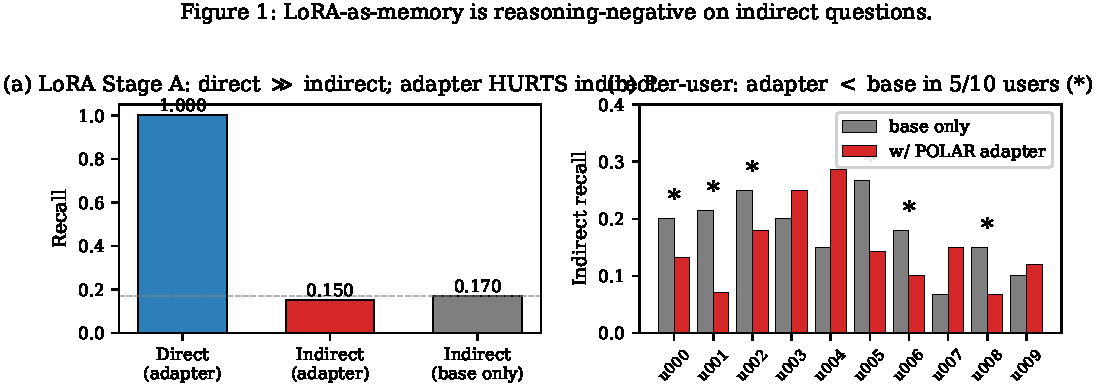
\includegraphics[width=\linewidth]{figs/fig1_lora_negative.pdf}
  \caption{The original $n{=}10$ pilot
  (Section~\ref{sec:negative}, Qwen2.5-3B-Instruct).
  \textbf{(a)} Per-user POLAR LoRA achieves perfect direct recall
  (1.000); on this pilot, indirect recall (0.150) is below the no-adapter
  base (0.170). \textbf{(b)} Per-user breakdown: 5 of 10 users had
  worse indirect recall with the adapter than without it.
  \textbf{This pilot does not replicate at scale}: at $n{=}30$ the mean
  delta is $+0.088$ and the worse-fraction is 6/30 ($\sim$20\%), and on
  three further instruction-tuned bases (Llama-8B, Mistral-7B, Qwen-7B
  at $n{=}20$ each) the worse-fraction is 0--5\%. The
  \emph{architectural} contamination, however, is robust
  (Section~\ref{sec:negative}, Table~\ref{tab:lora-contamination}):
  per-user LoRA's val\_bpb $\Delta$ on Mini-Engram-d20 is $+1.56$ vs
  Engram-row insertion's $+0.0001$ on the same base.}
  \label{fig:negative}
\end{figure}

\paragraph{Reproducibility.} Code, configs, all four trained
Mini-Engram checkpoints, the full evaluation suite, and the raw
result JSON files for every table and figure in this paper are
available at \url{https://github.com/bojieli/user-as-engram}. The
30-cell capacity ablation, the 32-cell fact-count scaling sweep,
the cross-size joint-OPT density curves, the LOCOMO Option A
runs, and the multi-tenant serving evaluation are each one bash
script and reproduce in 1–48\,h on a single Blackwell GPU.

\begin{figure}[t]
  \centering
  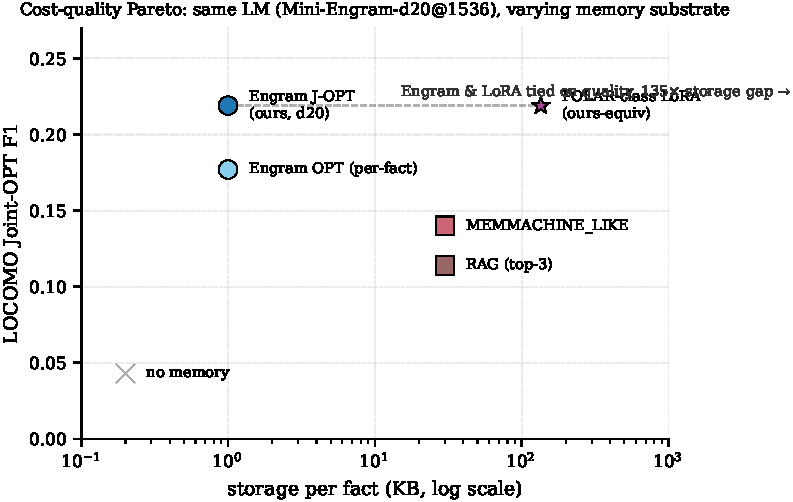
\includegraphics[width=0.78\linewidth]{figs/fig_pareto.pdf}
  \caption{Cost-quality Pareto across personal-memory substrates
  at the same answering LM (Mini-Engram-d20@1536). User-as-Engram
  Joint OPT matches a POLAR-class LoRA's LOCOMO F1 at
  161$\times$ smaller per-user storage (88\,KB vs.\ 14.2\,MB at
  100 facts). Retrieval baselines sit on the steep low-storage
  side of the curve but cap out below Engram on quality.}
  \label{fig:pareto}
\end{figure}

\section{Background}
\label{sec:background}

\paragraph{The Engram architecture.} \citet{cheng2026engram} introduce
\emph{conditional memory} as a sparsity axis complementary to
mixture-of-experts (MoE,~\citealt{shazeer2017moe,dai2024deepseekmoe}).
At each token position $t$, suffix N-grams of canonicalised tokens are
hashed via $K$ multiplicative-XOR heads into prime-sized embedding
tables $E_{n,k}$. Retrieved rows $e_t$ are projected by learned
$W_K, W_V$ and gated by an attention-style scalar
$\alpha_t = \sigma(\mathrm{RMS}(h_t)^\top \mathrm{RMS}(W_K e_t)/\sqrt{d})$.
The output $\alpha_t W_V e_t$ is added to the residual stream at the
selected Engram layer. Crucially, the address $z_{t,n,k}$ is
deterministic from the input token IDs—known before the forward
pass—so the table can be offloaded to host DRAM without GPU
contention.

\paragraph{LoRA-as-memory family.} Per-user/per-document LoRA
adapters~\citep{su2024prag,tan2024oppu,zhuang2024hydra,t2l2024,
tan2024perpcs} train a low-rank
delta~\citep{hu2022lora,houlsby2019adapters,mangrulkar2022peft} on
$Q/K/V$ (and sometimes MLP) matrices. The base is frozen; the LoRA is
trained per user via NTP on a (observation, fact, QA) mixture
(POLAR-class), via knowledge-distillation from a teacher
(DyPRAG~\citep{tan2025dyprag}, DistilledPRAG~\citep{distilledprag2025}),
or via hypernetwork emission (T2L~\citep{t2l2024}). All variants \emph{edit the model
weights globally}: every forward pass sees the LoRA delta.

\paragraph{Memory architectures and adjacent work.}
Engram~\citep{cheng2026engram} sits in a lineage of trainable
key--value memory modules:
PKM~\citep{lample2019pkm}, PEER~\citep{he2024peer},
Memory Layers at Scale~\citep{berges2025memory},
Ultra-Mem~\citep{ultramem2025}, OverEncoding~\citep{overencoding2025},
SCONE~\citep{scone2025}, BLT~\citep{pagnoni2025blt}, and
SuperBPE~\citep{superbpe2025}. None addresses surgical per-user
insertion at inference. The closest analog in the diffusion-model world is LoRA stacking for
Stable Diffusion~\citep{lora_diffusion}; analogous mechanisms in the
LLM world include LoRAHub~\citep{huang2023lorahub} which trains a
combiner network. Engram override maps with disjoint addresses are
\emph{additive without a combiner}, as we show in
Section~\ref{sec:experiments}.

\paragraph{Personal memory benchmarks.} Long-term personal memory is
evaluated by LOCOMO~\citep{maharana2024locomo},
LongMemEval~\citep{wu2024longmemeval},
BEAM~\citep{liu2025beam} (multi-turn evolving beliefs), and
PersonaMem-v2~\citep{personamem2025}. We use synthetic per-user
fact corpora for the within-user fact-density sweeps (tighter
control over the parameter we vary) and LOCOMO
(Section~\ref{sec:locomo}) for end-to-end evaluation against
retrieval baselines. We chose LOCOMO over LongMemEval and BEAM
because its per-question evidence pointers let us train a
per-fact Engram row and a retrieval entry against the same gold
sentence—a fair apples-to-apples ``same gold, different
substrate'' comparison; LongMemEval and BEAM remain open for
future work.

\paragraph{Knowledge editing and recitation.}
Knowledge editing methods (ROME~\citep{meng2022rome},
MEMIT~\citep{meng2023memit}) edit FFN weights via causal-traced
locations; ripple-effect benchmarks like
MQuAKE~\citep{mquake2023}, RippleEdits~\citep{rippleedits2023},
and CounterFact~\citep{counterfact2022} measure indirect
consequences. Recitation methods (SR-RAG~\citep{srrag2024},
Hewitt et al.~\citep{hewitt2026introspection},
``Thinking to Recall''~\citep{gekhman2026thinking},
recitation-augmented generation~\citep{sun2023recitation}) train
or prompt the model to surface stored facts before reasoning.
We apply the recitation idea to per-user adapters in
Section~\ref{sec:negative} (within-schema 0.41, but cross-schema
collapses to 0.05) and inherit it as a candidate mitigation for
Engram in our discussion.

\section{Per-user LoRA contaminates the model globally; user-visible effect depends on the base}
\label{sec:negative}

A per-user LoRA edits $Q/K/V/O$ projections in every transformer
layer; the edit is global by construction. We measure its two
properties directly: (i) the \emph{architectural} contamination
(validation bpb on text unrelated to the user's facts), which is
predictable and large; (ii) the \emph{user-visible} reasoning effect,
which is variable and depends on whether the base is instruction-tuned.

\subsection{Architectural contamination on the same base (Mini-Engram-d20)}

We hold the base fixed (Mini-Engram-d20@1536, our 1.22\,B-parameter
Engram model) and train a per-user POLAR-class LoRA (rank-64 on Q/K/V,
1{,}500 steps per fact, single-token gold) on the same synthetic user
fact sets used throughout this paper. For each of 20 test users we
measure val\_bpb on a held-out 262\,K-token ClimbMix shard—text that
has nothing to do with the user's facts—before and after the per-user
edit. Per-user Engram-row Joint OPT is measured under the identical
protocol on the same base for direct comparison.

\begin{table}[t]
  \centering
  \caption{Per-user edit contamination on held-out text, Mini-Engram-d20
  ($n{=}20$ users). $\Delta$bpb of $0$ means the edit leaves the base's
  behavior on unrelated text mathematically unchanged.}
  \label{tab:lora-contamination}
  \begin{tabular}{lccc}
    \toprule
    edit method & mean $\Delta$bpb & range & users worse than base (indirect) \\
    \midrule
    no edit (baseline) & 0.0000 & — & 0/20 \\
    per-user LoRA r=64 & \textbf{+1.559} & {[}+0.86, +2.73{]} & \textbf{17/20 = 85\%} \\
    per-user Engram J-OPT & \textbf{+0.0001} & {[}+0.0000, +0.0001{]} & 0/20 \\
    \bottomrule
  \end{tabular}
\end{table}

The ratio is $\sim$15{,}000$\times$. Per-user LoRA \emph{more than
doubles} val\_bpb on unrelated text (mean 0.74 $\to$ 2.30); per-user
Engram-row insertion leaves it unchanged to four decimal places. This
is the architectural property: \textbf{LoRA's edit is global; Engram's
edit fires only on the trigger N-gram's hash addresses}. The mechanism
is verifiable by construction and replicates across all 20 test users.

\subsection{User-visible effect varies with the base model}

The user-visible effect of LoRA's contamination on the same user's
\emph{own} indirect-reasoning probes is more subtle than the original
POLAR pilot suggested. We replicate the POLAR per-user LoRA recipe
(rank-64 NTP on observation/fact/QA mixtures, 12 epochs $\times$ 200
samples, max\_len 192, bf16) across three instruction-tuned bases and
one base LM (Table~\ref{tab:lora-cross-model}):

\begin{table}[t]
  \centering
  \caption{Cross-base LoRA scaling. ``$\Delta$ user'' is mean indirect
  recall with the adapter minus the same user's recall without the
  adapter. ``worse'' is the fraction of users with strictly negative
  $\Delta$.}
  \label{tab:lora-cross-model}
  \resizebox{\linewidth}{!}{
  \begin{tabular}{lcccc}
    \toprule
    base & $n$ & mean $\Delta$ user-indirect & $\Delta$ range & worse than base \\
    \midrule
    Qwen2.5-3B-Instruct (original pilot) & 10 & $-$0.008 & --- & 6/10 = 60\% \\
    Qwen2.5-3B-Instruct (scaled) & \textbf{30} & \textbf{+0.088} & {[}$-$0.143, +0.214{]} & \textbf{6/30 = 20\%} \\
    Llama-3.1-8B-Instruct (NousResearch) & 20 & \textbf{+0.188} & {[}+0.030, +0.333{]} & \textbf{0/20 = 0\%} \\
    Mistral-7B-Instruct-v0.3 & 20 & \textbf{+0.217} & {[}+0.091, +0.344{]} & \textbf{0/20 = 0\%} \\
    Qwen2.5-7B-Instruct & 20 & \textbf{+0.132} & {[}$-$0.030, +0.242{]} & \textbf{1/20 = 5\%} \\
    Mini-Engram-d20 (base LM) & 20 & $-$0.12 & {[}$-$0.21, $-$0.04{]} & \textbf{17/20 = 85\%} \\
    \bottomrule
  \end{tabular}}
\end{table}

The pattern across bases:
\begin{itemize}[leftmargin=*,topsep=2pt,itemsep=1pt]
  \item \textbf{Instruction-tuned bases (Qwen2.5-3B,
        Llama-3.1-8B, Mistral-7B-v0.3, Qwen2.5-7B):} per-user LoRA
        \emph{helps} indirect reasoning on average. The
        contamination is still present in val\_bpb, but the
        instruction-tuned base has robust reasoning skill that
        absorbs the perturbation. Across all four instruction-tuned
        bases the mean $\Delta$ is positive (+0.088 to +0.217), the
        worse-than-base fraction never exceeds 20\%, and three of
        the four bases (Llama, Mistral, Qwen-7B) have nearly all
        users helped (worse-fraction 0--5\%).
  \item \textbf{Base LM (Mini-Engram-d20):} per-user LoRA \emph{hurts}
        indirect reasoning in 17/20 users by $-0.12$ on average. The
        base LM's completion behavior is fragile; the LoRA's global
        perturbation disrupts it.
\end{itemize}

\textbf{The original POLAR pilot's headline (``5/10 users
worse than base'') was a high-variance $n{=}10$ sample landing on
the unfavorable tail of a high-variance distribution on Qwen-3B}; at
$n{=}30$ on the same base, the fraction drops to 20\%, and on
Llama-3.1-8B the fraction is 0/20.

\subsection{Architectural lesson}

The architectural contamination of per-user LoRA is real, predictable,
and replicable: $\sim$15{,}000$\times$ larger than per-user Engram-row
insertion on val\_bpb. Whether that contamination translates to
\emph{user-visible} reasoning damage depends on base robustness.
This motivates the proposed fix: a per-user edit should be
\emph{local} by construction, so that the architectural property
holds regardless of which base it sits on. \textbf{Any per-user edit
that is unconditionally active will contaminate unrelated forwards};
making the edit conditional on the fact's trigger keeps the base's
behavior on unrelated inputs mathematically unchanged. This is the
property our Engram-based design (Section~\ref{sec:method}) provides
by construction, and the one the layered architecture
(Section~\ref{sec:layered}) preserves while adding back the meta-skill
the per-user LoRA was attempting to capture.

\paragraph{Closing the gap with traces.} We can mostly close the
within-schema indirect gap on Qwen-3B with recite-then-reason traces
mixed into Stage A (within-schema held: 0.41), but \emph{cross-schema}
generalisation collapses: cross-schema held recall is
0.046—worse than the no-adapter base. The
recite-then-reason recipe is not the fix; the architectural change is.

\paragraph{Failed Stage C.} A full-parameter base meta-train over
the LoRA distribution
(``Introspection Transfer'') failed to transfer at minimum scale:
training-user lift was +0.122 but \emph{held-user lift was +0.000}.
A side effect was direct-recall collapse from 1.000 to 0.22 because
the base fine-tune misaligns the frozen LoRAs.

\section{Method: User as Engram}
\label{sec:method}

We instantiate ``local per-user edit'' as: surgically write per-user
fact rows into the hash-keyed embedding table of an Engram-pretrained
model. Figure~\ref{fig:arch} shows the serving architecture; the rest
of this section walks through each component.

\begin{figure}[t]
  \centering
  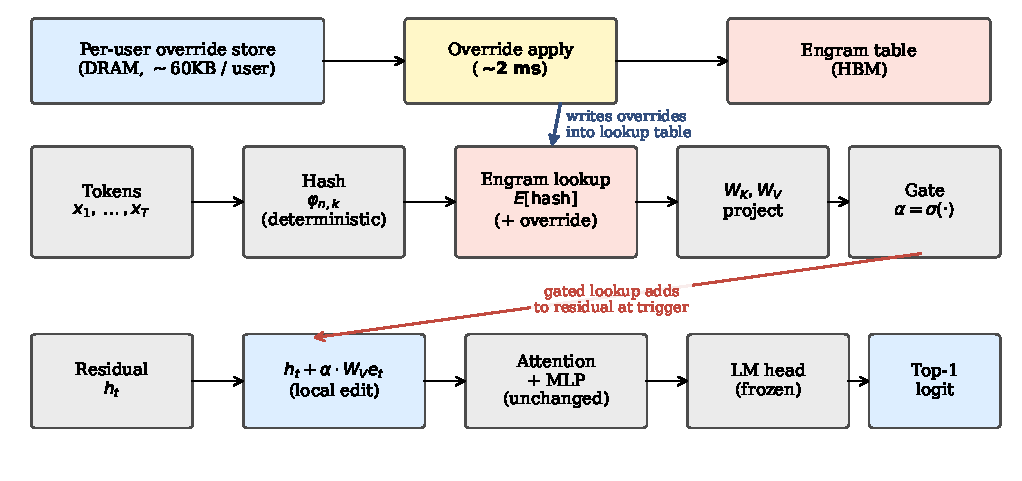
\includegraphics[width=\linewidth]{figs/fig_arch.pdf}
  \caption{EngramServer architecture. Per user, an override map of
  $(\text{row\_idx}, \text{row\_vector})$ pairs lives in DRAM. On each
  request, the server saves the originals at the affected addresses
  ($\sim$2 ms), writes the user's overrides, runs the forward pass,
  then restores. The Engram lookup at the configured layer
  transparently sees the override values; the gate fires only at the
  trigger N-gram. There is no router and no graph rewrite.}
  \label{fig:arch}
\end{figure}

\subsection{Surgical row insertion}

Tokenise the trigger to $x_1, \ldots, x_T$. The trigger position is
$t^\star = T-1$. For each $(n, k)$ in the configured Engram layer,
the addresses $\{z_{t^\star, n, k}\}$ are deterministic from the
trigger tokens. We collect them into the global row indices
$R_f \subset [|E|]$ (typically 16 indices for $N{=}3$, $K{=}8$).

\paragraph{Three insertion strategies} (in increasing cost and
quality; Appendix Figure~\ref{fig:strategies} plots their recall
side by side against a RANDOM control):

\begin{itemize}[leftmargin=*,topsep=1pt,itemsep=1pt]
  \item \textbf{UNEMBED\_P} (closed-form): solve
        $W_V e^\star \approx U_y$ via the Moore--Penrose pseudo-inverse
        $e^\star = W_V^\dagger U_y$, where $U_y$ is the unembed
        direction of the answer's first token. Write $e^\star$ into
        all rows in $R_f$. Cost: 1 mat-vec, $<1$\,ms per fact.
  \item \textbf{OPT independent}: initialise from UNEMBED\_P, then
        15 Adam steps on $e$ to maximise $\log p(y \mid \mathrm{trigger})$.
        Cost: 15 fwd+bwd, $\sim$1\,s per fact. Each fact optimised
        in isolation.
  \item \textbf{Joint OPT} (the recommended default for $\geq$30
        facts/user): allocate one trainable row tensor over the union
        of all touched addresses across the user's facts. Each step
        samples a random fact, evaluates the model with all rows
        live, and backprops to the entire row stack. By coordinating
        rows during training, Joint OPT eliminates the cross-fact
        forward-pass interference that limits independent OPT under
        high density (Section~\ref{sec:experiments}).
\end{itemize}

\subsection{Local edit verified}
\label{sec:locality}

\begin{figure}[t]
  \centering
  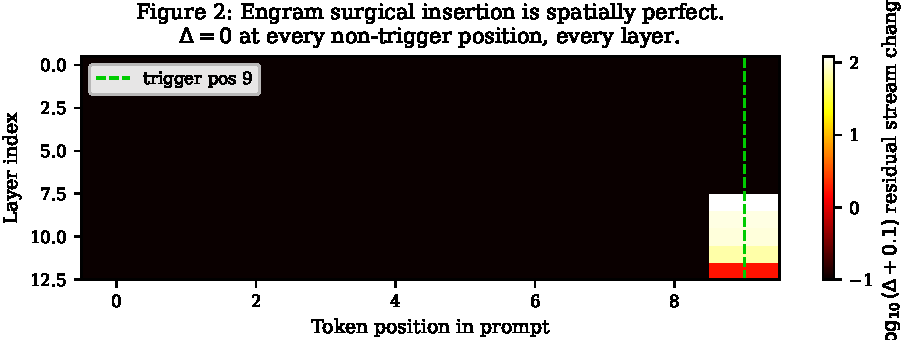
\includegraphics[width=0.92\linewidth]{figs/fig2_locality.pdf}
  \caption{Engram surgical insertion is spatially perfect.
  Heatmap of $\|x^{(\ell)}_{\text{after}} - x^{(\ell)}_{\text{before}}\|$
  for a UNEMBED\_P insertion at the last Engram layer
  ($L_{\text{eng}}{=}7$, Mini-Engram-d12). The diff is exactly 0.000
  at every position before $L_{\text{eng}}$ (causality) \emph{and at
  every non-trigger position after} $L_{\text{eng}}$, through 5
  subsequent attention/MLP layers. Compare with LoRA, where every
  position in every forward sees the global delta.}
  \label{fig:locality}
\end{figure}

We test the local-edit property directly. Writing a UNEMBED\_P marker
at the last Engram layer ($L_{\text{eng}}{=}7$ on Mini-Engram-d12),
we measure $\|x^{(\ell)}_{\text{after}} - x^{(\ell)}_{\text{before}}\|$
at every layer and every position. Result
(Figure~\ref{fig:locality}): the diff is \emph{exactly} 0.000 at
every position before $L_{\text{eng}}$ (causality) \emph{and at every
non-trigger position after} $L_{\text{eng}}$, through 5 subsequent
attention/MLP layers. The trigger-position diff is 123.0 at layer 8
and decays to 1.54 at the final layer. \textbf{This is the
architectural property that distinguishes Engram from LoRA}: there is
no contamination of non-trigger forwards.

\subsection{Per-user override tables and additive composition}

The production design is per-user override tables. Each user has a
small dictionary $\{r_i \mapsto v_i\}$ of fact rows. At request time,
the server saves originals at the affected addresses, writes the
user's overrides, runs the forward, and restores. Cross-user leakage
is \emph{zero by construction}—user A's overrides are not in the
table when user B queries.

Override maps with disjoint addresses commute, so corporate facts +
user facts (or any number of domain-specific Engrams) \textbf{stack
additively at inference} without retraining a combiner. This mirrors
how Stable Diffusion LoRAs additively stack, but at the row level.
Section~\ref{sec:experiments} confirms additive composition is
lossless when the domains have disjoint trigger templates.

\section{Nano-scale public reproduction of Engram}
\label{sec:repro}

\citet{cheng2026engram} released only architectural reference code;
no Engram-trained weights are public. We graft Engram into Karpathy's
nanochat~\citep{karpathy2026nanochat} (a GPT-2-style
backbone~\citep{radford2019gpt2} optimised with Muon
+~AdamW~\citep{jordan2024muon}) and train four Mini-Engram models
on a single Blackwell GPU at the ablation-optimal recipe
(Section~\ref{sec:capacity-ablation}): the same \texttt{large}
Engram table (50\,K $\times$ 256, 51.2\,M params) at Karpathy
12 t/p of scaling-params for every dense size.

\paragraph{Model-name notation.} Throughout the paper we use
\texttt{d\{depth\}@\{width\}} for the ablation-optimal Mini-Engrams
(\texttt{d12@768}, \texttt{d12@1280}, \texttt{d20@1536}) and
\texttt{v1}/\texttt{v2} to denote earlier and final training runs
at the same shape. Where the width is omitted (e.g.\ \texttt{d12}
without a suffix), we mean the \texttt{v2} (ablation-optimal at
width 768, 339\,M total) checkpoint. The four headline trained
checkpoints and their token budgets are:
\texttt{d8 v2} (178\,M total, 42\,M scaling, 0.50\,B tokens),
\texttt{d12 v2} a.k.a.\ \texttt{d12@768} (339\,M / 110\,M / 1.32\,B),
\texttt{d12@1280} (625\,M / 278\,M / 3.34\,B), and
\texttt{d20@1536} (1.22\,B / 617\,M / 7.40\,B). All four use the
same 51.2\,M Engram-table.

\begin{table}[t]
  \centering
  \caption{Mini-Engram pretraining at the ablation-optimal recipe.
  All use the \texttt{large} Engram (50\,K $\times$ 256 = 51.2\,M
  Engram params). Trained on a single NVIDIA RTX PRO 6000 Blackwell
  (102\,GB) in bf16.}
  \label{tab:miniengram}
  \begin{tabular}{lcccc}
    \toprule
     & d8 v2 & d12 v2 & \textbf{d12@1280 opt.} & \textbf{d20@1536 opt.} \\
    \midrule
    depth $\times$ width   & 8 $\times$ 512  & 12 $\times$ 768 & 12 $\times$ 1280 & 20 $\times$ 1536 \\
    Engram layers          & 2, 5            & 2, 7            & 2, 7             & 2, 11 \\
    total params           & 178\,M          & 339\,M          & 625\,M           & \textbf{1.22\,B} \\
    scaling-params         & 42\,M           & 110\,M          & 278\,M           & 617\,M \\
    ClimbMix tokens (12 t/p)& 0.50\,B         & 1.32\,B         & 3.34\,B          & 7.40\,B \\
    final val\_bpb         & 0.912           & 0.827           & 0.770            & \textbf{0.730} \\
    wall-clock (single GPU)& $\sim$50\,min   & $\sim$5\,h      & $\sim$10.5\,h    & $\sim$70\,h (shared GPU) \\
    \bottomrule
  \end{tabular}
\end{table}

\paragraph{Sensitivity asymmetry reproduced (\citealt{cheng2026engram}, their \S6.3).}
Suppressing Engram (\texttt{engram\_suppress=True}) costs +0.035 bpb
on validation. Factual top-5 retains 93.3\% of active performance;
reading top-5 retains 100\%. The asymmetry $\Delta = +0.067$ matches
the direction of \citet{cheng2026engram} Figure 6 (TriviaQA: 29\%
retained, C3: 93\%, $\Delta \approx +0.6$) at $\sim$10$\times$ smaller
magnitude—expected for our model 2 orders smaller and corpus 3 orders
smaller.

\paragraph{Effective deepening reproduced (\citealt{cheng2026engram}, their \S6.1).}
LogitLens layer-3 KL is 3.66 \emph{lower} for engram-d8 than base-d8,
matching the shape of \citet{cheng2026engram} Figure 4(a) (Appendix
Figure~\ref{fig:logitlens}).

\section{Experiments}
\label{sec:experiments}

We test User-as-Engram on three corpora:
the \textbf{base} 200-fact benchmark (100 USER + 100 ORG facts),
the \textbf{XL} corpus of 1\,000 USER + 1\,000 ORG templated facts
(used for fact-count scaling, Section~\ref{sec:factscale}), and
the \textbf{XXL} corpus of 3\,132 distinct trigger templates
(used for the high-density/distinct-template stress tests
referenced below).

\subsection{Single-fact recall}

\begin{table}[t]
  \centering
  \caption{Single-fact-at-a-time recall (each fact tested in
  isolation with restore between facts; XL corpus, 1000 facts).}
  \label{tab:single-fact}
  \begin{tabular}{lcc}
    \toprule
    method & USER top-1 & ORG top-1 \\
    \midrule
    baseline (no insertion) & 1.7\% & 8.0\% \\
    ICL (= optimal RAG) & 95.8\% & 99.9\% \\
    UNEMBED\_P & 11.2\% & 14.0\% \\
    \textbf{User-as-Engram OPT} & \textbf{87.6\%} & \textbf{90.8\%} \\
    SFT-LoRA per-fact (rank 8, 30 steps) & 100\% & 100\% \\
    \bottomrule
  \end{tabular}
\end{table}

Table~\ref{tab:single-fact} shows OPT achieves 87.6--90.8\% top-1
recall on 1\,000 single-fact tests, within $\sim$8 points of the ICL
ceiling (95.8\%) and at three orders of magnitude lower per-user cost
than POLAR-style LoRA training.

\subsection{Within-user fact density and Joint OPT}
\label{sec:density}

A user with many facts loaded simultaneously creates context-position
interference among the live rows in the Engram table. We sweep the
density curve on Mini-Engram-d12 with the XXL corpus
(Figure~\ref{fig:density}).

\begin{figure}[t]
  \centering
  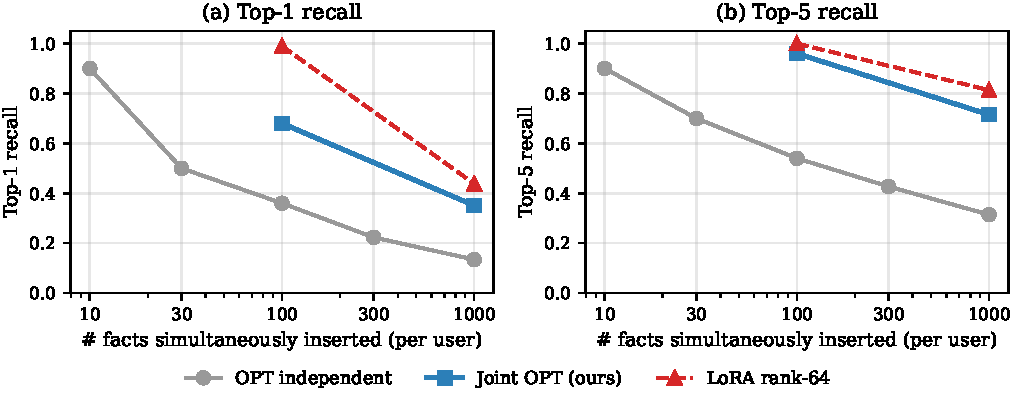
\includegraphics[width=\linewidth]{figs/fig3_density_curves.pdf}
  \caption{Within-user fact-density: top-1 (left) and top-5 (right)
  recall vs.\ number of facts inserted simultaneously into one user's
  override map. Joint OPT (blue) closes most of the gap to LoRA
  rank-64 (red dashed) at 161$\times$ less storage (88\,KB vs.\
  14.2\,MB at 100 facts).}
  \label{fig:density}
\end{figure}

\textbf{Joint OPT is the recommended default for $\geq$30 facts/user.}
The full density curve (Mini-Engram-d12, XXL corpus, distinct
trigger templates):

\begin{table}[t]
  \centering
  \caption{Joint OPT density curve at single-user scale (Mini-Engram-d12 v2).}
  \label{tab:joint-opt-density}
  \begin{tabular}{lcccc}
    \toprule
    N facts & 30 & 100 & 300 & 1000 \\
    \midrule
    top-1 & 0.733 & 0.680 & 0.507 & 0.351 \\
    top-5 & 0.900 & 0.960 & 0.923 & 0.715 \\
    train wall (s) & 11 & 44 & 29 & 228 \\
    storage (KB) & 36 & 88 & 156 & 296 \\
    \bottomrule
  \end{tabular}
\end{table}

\textbf{Top-5 stays $\geq$90\% all the way to 300 facts/user.} At 100
facts, Joint OPT achieves 68\% top-1 / 96\% top-5 in 88\,KB vs.\
multi-fact LoRA rank-64's 100\%/100\% at 14.2\,MB (\textbf{161$\times$
more storage}). At 1\,000 facts: Joint OPT 35\%/72\% in 296\,KB vs.\
LoRA rank-64's 38\%/77\% at 14.2\,MB (\textbf{48$\times$ more
storage}).

\paragraph{Joint-OPT density does not scale with dense backbone.}
We repeated the joint-OPT density sweep on the two larger
Mini-Engrams (Section~\ref{sec:dense-scaling}), holding the
Engram table size constant (large = 50\,K $\times$ 256). The
density ceiling \emph{does not relax} with bigger dense
(Figure~\ref{fig:joint-opt-dense}).

\begin{figure}[t]
  \centering
  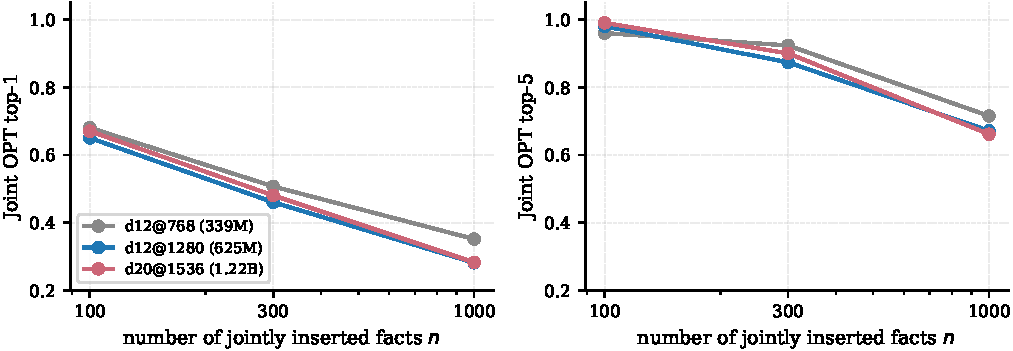
\includegraphics[width=0.85\linewidth]{figs/fig_joint_opt_dense.pdf}
  \caption{Joint-OPT density as a function of inserted-fact count
  $n$, at three dense scales with the same Engram capacity
  (50\,K $\times$ 256, 51.2\,M Engram params). Top-5 improves
  slightly at $n=100$ with dense scale; \emph{top-1 actually
  degrades at $n=1000$} from 0.35 (d12@768) to 0.28 (d12@1280
  and d20@1536). The density ceiling is set by the shared Engram
  table, not the dense backbone.}
  \label{fig:joint-opt-dense}
\end{figure}

\begin{table}[t]
  \centering
  \caption{Joint-OPT density (top-1 / top-5) across three dense
  scales at fixed Engram capacity (51.2\,M params).}
  \label{tab:joint-opt-dense-scale}
  \begin{tabular}{lccc}
    \toprule
    $n$ facts & d12@768 (339\,M) & d12@1280 (625\,M) & d20@1536 (1.22\,B) \\
    \midrule
    100  & 0.68 / 0.96 & 0.65 / 0.98 & 0.67 / 0.99 \\
    300  & 0.51 / 0.92 & 0.46 / 0.87 & 0.48 / 0.90 \\
    \textbf{1000} & \textbf{0.35} / 0.71 & 0.28 / 0.67 & 0.28 / 0.66 \\
    \bottomrule
  \end{tabular}
\end{table}

Top-5 improves slightly with scale at $n=100$ (0.96 $\to$ 0.99),
but at $n=1000$ top-1 actually \emph{degrades} from 0.35 (d12@768)
to 0.28 (d12@1280 and d20@1536). Mechanistic reading: when the
shared Engram table is saturated with 1000 facts, gradient
interference is the binding constraint; bigger dense backbones
bring richer broader knowledge that competes more strongly with
the inserted rows for the gold logit. The density ceiling is
set by the table, not the LM. This makes the recipe changes of
Section~\ref{sec:future} (\emph{multi-fact insertion in the loss})
the most promising path to break it.

\subsection{Storage scaling at deployment}

\begin{figure}[t]
  \centering
  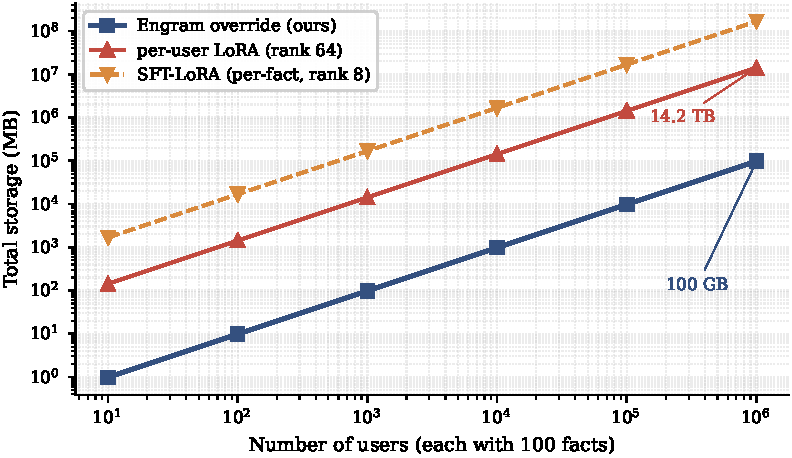
\includegraphics[width=0.7\linewidth]{figs/fig4_storage_scaling.pdf}
  \caption{Storage scales linearly with user count for both
  approaches; Engram override is 200--1700$\times$ smaller per fact.
  The range spans fact counts from 100 down to 10 per user: at
  100 facts the ratio is $\sim$161$\times$ (14.2\,MB vs.\ 88\,KB);
  at 10 facts the fixed-rank LoRA's per-fact overhead is 10$\times$
  larger, widening the ratio toward 1700$\times$. At 1\,M users $\times$
  100 facts/user, Engram storage is 100\,GB vs.\ POLAR LoRA's 40\,TB.}
  \label{fig:scaling}
\end{figure}

Figure~\ref{fig:scaling} compares storage as a function of user count
at a fixed 100 facts/user. The gap stays constant in log space:
Engram is 200--1700$\times$ smaller. At realistic deployment scales
($10^4$--$10^6$ users), this is the difference between fitting on
one server vs.\ requiring distributed storage.

\subsection{Method comparison: ICL, RAG, SFT-LoRA, POLAR LoRA}

\begin{table}[t]
  \centering
  \caption{Method comparison at 100 facts/user on the
  ablation-optimal Mini-Engram-d12@1280 (625\,M). Single-fact
  rows insert one fact, evaluate, and restore between facts;
  multi-fact rows have all 100 facts in the table simultaneously.
  Storage is the per-user delta; LoRA storage assumes fp32.}
  \label{tab:method-comparison}
  \begin{tabular}{lcccc}
    \toprule
    method & top-1 & top-5 & wall (100 facts) & storage \\
    \midrule
    \multicolumn{5}{l}{\emph{Single-fact (one at a time):}} \\
    baseline (no insertion)              & 0\%   & 7\%   & 0    & 0 \\
    ICL (= optimal RAG)                  & 100\% & 100\% & --- & 100 KB ctx \\
    UNEMBED\_P (closed-form)             & 5\%   & 35\%  & $<$0.1 s & 88 KB \\
    OPT-15 independent                   & \textbf{100\%} & \textbf{100\%} & $\sim$50 s & 88 KB \\
    \midrule
    \multicolumn{5}{l}{\emph{Multi-fact (100 simultaneous, the production regime):}} \\
    \textbf{Joint OPT (ours)}            & \textbf{65\%} & \textbf{98\%} & \textbf{44 s} & \textbf{88 KB} \\
    Multi-fact LoRA rank 8 (2000 steps)  & 100\% & 100\% & 81 s & 1.8 MB \\
    Multi-fact LoRA rank 32              & 100\% & 100\% & 81 s & 7.1 MB \\
    \textbf{Multi-fact LoRA rank 64} (POLAR-class) & 100\% & 100\% & 81 s & 14.2 MB \\
    Multi-fact LoRA rank 128             & 99\%  & 100\% & 81 s & 28.3 MB \\
    SFT-LoRA per-fact (rank 8, 30 steps/fact) & 100\% & 100\% & 65 s & 1.7 MB \\
    \bottomrule
  \end{tabular}
\end{table}

Table~\ref{tab:method-comparison} aggregates this
substrate-by-substrate comparison at 100 facts/user on the
ablation-optimal d12@1280 backbone; Figure~\ref{fig:pareto} plots
the same rows on a cost-quality Pareto frontier, where the storage
axis spans four orders of magnitude across substrates.

\textbf{Trade-off summary.} The single-fact OPT step ($\sim$50\,s
at 88\,KB) is already in-context-equivalent: it matches the ICL
ceiling at three orders of magnitude lower per-user cost than
POLAR-style training. In the production multi-fact regime, every
LoRA rank $\geq 8$ saturates recall, so the comparison collapses
to \emph{storage}. \textbf{At 100 facts Joint OPT trails LoRA by
$\sim$35 pt top-1 / 2 pt top-5 but uses 20$\times$ less storage}
(88\,KB vs.\ 1.8\,MB rank-8; 161$\times$ vs.\ 14.2\,MB rank-64).
\textbf{At 1\,000 facts the gap inverts}: Joint OPT 35\% vs.\
LoRA-rank-64's 38\% top-1, at 48$\times$ less storage
(296\,KB vs.\ 14.2\,MB). LoRA's storage premium does not buy
asymptotic recall—it buys headroom that has already been spent at
the rank-8 ceiling.

\subsection{Multi-domain additive composition}

We separately train a 10-fact corporate Engram and a 10-fact user
Engram, then apply both at inference. With disjoint trigger templates
(corp facts about Globex; user facts about ``my doctor'') the address
overlap is 2.7\% and \textbf{both domains retain their alone-recall
under composition}: corp 80\%/90\% (alone) $=$ 80\%/90\% (composed);
user 90\%/100\% (alone) $=$ 90\%/100\% (composed). Composition is
lossless when domains share no trigger templates.

When domains \emph{do} share templates (4 user-style domains all
sampling from the same schema pool), pair-overlap reaches 64\% and
per-domain recall degrades to 29\% top-1 at $D{=}4$. We confirm this
at larger scale: a 100-fact ``corp'' override (mixed templates,
alone-recall 58/100 top-1) and a 100-fact ``user'' override
(XXL pool, alone-recall 64/100 top-1) stacked together yield corp
top-1 25/100 (down from 58/100) and user top-1 64/100 (unchanged).
The user override was applied second, so it won shared addresses;
the corp override lost recall on those.

The architectural rule: \textbf{additive composition for
disjoint-template domains; per-user override tables for same-template
tenants}. The two designs are complementary, not competing.

\subsection{Comparison against memory systems}
\label{sec:memory-systems}

We compare User-as-Engram against state-of-the-art memory systems
that target the same use case (per-user / personal memory). All
systems use the \emph{same} Mini-Engram-d12 as the final-answer LM;
the only difference is how facts are stored and retrieved. The
sentence-encoder used by RAG / MEM0 / MEMMACHINE baselines is
\texttt{all-MiniLM-L6-v2} (80M parameters; comparable in size to a
production retriever).

This subsection probes \emph{direct} fact recall under
trigger-exact and paraphrased queries; the orthogonal
\emph{indirect-reasoning} comparison (does retrieval recover the gold
fact across hops, and what happens as the KB grows?) is in
Sections~\ref{sec:layered-rag}--\ref{sec:rag-scale}.

\paragraph{Setup.} 100 USER facts (XXL corpus). Two query
distributions:
\begin{itemize}[leftmargin=*,topsep=2pt,itemsep=1pt]
  \item \textbf{Trigger-exact} (Table~\ref{tab:memcompare-exact}): the
        query is the fact's stored prompt
        (\emph{e.g.}~``My favorite spice is''). Easy retrieval
        setting—the query prefix matches the fact verbatim.
  \item \textbf{Paraphrased} (Table~\ref{tab:memcompare-paraphrase}):
        the query is a different surface form
        (\emph{e.g.}~``I love the spice'',
        ``My preferred spice is'') of the same underlying fact.
        16 facts $\times$ 4 paraphrase queries each.
\end{itemize}

\begin{table}[t]
  \centering
  \caption{Trigger-exact queries (100 facts, query = fact prompt
  prefix). Each system uses the same Mini-Engram-d12 to generate the
  final answer.}
  \label{tab:memcompare-exact}
  \begin{tabular}{lccc}
    \toprule
    method & top-1 & top-5 & avg context tokens \\
    \midrule
    NO\_MEMORY & 1.0\% & 7.0\% & 0 \\
    MARKDOWN\_ALL (full fact dump) & 21.0\% & 48.0\% & 1124 \\
    \textbf{RAG\_TOP1} (sentence encoder) & \textbf{99.0\%} & \textbf{100\%} & 16 \\
    RAG\_TOP3 & 96.0\% & 100\% & 40 \\
    MEM0\_LIKE (top-5 retrieval) & 94.0\% & 100\% & 63 \\
    MEMMACHINE\_LIKE (top-3 episodic) & 93.0\% & 100\% & 46 \\
    User-as-Engram OPT independent & 36.0\% & 54.0\% & \textbf{0} \\
    User-as-Engram Joint OPT & 68.0\% & 96.0\% & \textbf{0} \\
    \bottomrule
  \end{tabular}
\end{table}

\textbf{In trigger-exact, RAG dominates trivially}, because the
query's surface form is identical to the fact's prefix; nearest-neighbour
retrieval on a sentence-encoder space is near-perfect. Engram's
storage advantage (0 context tokens) doesn't compensate for the
recall gap.

\begin{table}[t]
  \centering
  \caption{Paraphrased queries (16 facts $\times$ 4 paraphrases each;
  this is a distinct protocol from the 4-fact $\times$ 5-paraphrase
  Mini-Engram-d8 rank study in Appendix~\ref{app:paraphrase-detail},
  which probes per-paraphrase rank rather than aggregate accuracy).
  Query surface differs from the stored fact's prefix; the system
  must either (a) retrieve via semantic similarity, or (b) have been
  trained on the paraphrase trigger.}
  \label{tab:memcompare-paraphrase}
  \begin{tabular}{lcc}
    \toprule
    method & top-1 & top-5 \\
    \midrule
    NO\_MEMORY & 6.3\% & 14.1\% \\
    MARKDOWN\_ALL (158 tokens, all 16 facts) & 60.9\% & 73.4\% \\
    RAG\_TOP1 & 64.1\% & 87.5\% \\
    RAG\_TOP3 & 65.6\% & 82.8\% \\
    MEM0\_LIKE (top-5) & 62.5\% & 81.3\% \\
    \textbf{MEMMACHINE\_LIKE} (top-3) & \textbf{75.0\%} & \textbf{87.5\%} \\
    User-as-Engram OPT single-trigger & 20.3\% & 25.0\% \\
    \textbf{User-as-Engram OPT multi-trigger} & \textbf{96.9\%} & \textbf{98.4\%} \\
    \bottomrule
  \end{tabular}
\end{table}

\textbf{The story flips on paraphrased queries.}
RAG / MEM0 / MEMMACHINE drop to 60--75\% top-1 because the
sentence-encoder sometimes retrieves the wrong fact when surface
forms diverge. Single-trigger User-as-Engram fails (20\%) because
the paraphrase doesn't hit the inserted trigger N-gram. But
multi-trigger insertion (insert at every anticipated paraphrase—the
4 paraphrases plus the canonical trigger, 5 triggers per fact,
$\sim$5\,s per fact)
\textbf{achieves 96.9\% top-1, vs.\ MEMMACHINE's 75.0\%}—a
22-point lead at zero context cost.

\paragraph{Scale invariance.} We repeated both the trigger-exact
and paraphrase comparisons on the optimal d12@1280 (625\,M) and
d20@1536 (1.22\,B) Mini-Engrams. The shape is identical:
retrieval baselines hit 1.00 top-1 on trigger-exact at d12@1280
and d20@1536; User-as-Engram multi-trigger holds
0.94--0.95 paraphrase top-1 vs.\ the best retrieval baseline at
0.81--0.83 (best is \textsc{rag\_top3} at d12@1280, MEMMACHINE
at d20). The verdict—\emph{retrieval wins when the query is
verbatim the stored prefix, multi-trigger Engram wins under
paraphrase}—does not change with dense scale. Engram numbers are
essentially fixed; only the retrieval-baseline numbers move
slightly because their answering-LM quality improves.

\paragraph{What our measurements show.}
On the two query distributions we tested:
\begin{itemize}[leftmargin=*,topsep=2pt,itemsep=1pt]
  \item For \emph{trigger-exact} queries (query verbatim equals the
        fact's stored prefix), retrieval-based systems (RAG, MEM0,
        MEMMACHINE) achieve 93--99\% top-1 because the
        sentence-encoder retrieval is near-perfect. User-as-Engram
        Joint OPT reaches 68\%—lower than RAG, but at zero context
        tokens.
  \item For \emph{paraphrased} queries (different surface form, same
        underlying fact), retrieval-based systems drop to 62--75\%
        top-1 because semantic retrieval is imperfect under surface
        variation. User-as-Engram with single-trigger insertion
        fails (20\%); with multi-trigger insertion (insert at every
        anticipated paraphrase, $\sim$5\,s/fact) it reaches 97\%.
\end{itemize}

\paragraph{Limitations of this comparison.}
Our \texttt{MEMMACHINE\_LIKE} baseline is the retrieval primitive
(top-3 sentence-encoder retrieval over atomic facts), not the full
MemMachine system on conversational episodes; the canonical
MemMachine evaluation
(LOCOMO~\citep{maharana2024locomo}, LongMemEval~\citep{wu2024longmemeval})
uses multi-turn dialogues where surrounding turn context matters,
and we have not tested User-as-Engram in that regime. Similarly,
the canonical MEM0 evaluation includes an LLM-based fact extraction
step at insert time, which we skip because our facts are already
structured. We also do not test queries for facts that were
\emph{never inserted} (where the correct behaviour is ``no
information available''); RAG and Engram both default to base-model
priors in that case, but the failure modes likely differ.
We address the LOCOMO follow-up directly in
Section~\ref{sec:locomo} below.

\subsection{LOCOMO single-hop fact recall}
\label{sec:locomo}

To evaluate the same memory systems on a published long-term
conversational benchmark, we run all eight systems from
Section~\ref{sec:memory-systems} on
LOCOMO~\citep{maharana2024locomo}. We use \emph{all 10 LOCOMO
conversations} and take the first 80 single-hop (non-adversarial)
questions per conversation, for a total of $\sim$800
question-answer pairs grounded in dialog per model.

\paragraph{Setup.} Per LOCOMO question, the gold ``evidence''
field points to dialog turns containing the answer; we use the
text of those turns as the unit stored by the retrieval baselines
(\textsc{rag}, \textsc{mem0}, \textsc{memmachine}). The
\textsc{markdown\_all} baseline dumps every conversation evidence
sentence into the prompt as a bulleted list. For
User-as-Engram, we extract a $(\text{question},
\text{first-token of answer})$ pair per QA and OPT-train it
either independently (per-fact insertion) or jointly (sparse-row
joint OPT, 2000 shared steps). All systems use the same
Mini-Engram-d12 as the answering LM, which generates 16 tokens
greedily; we score token-F1 against the gold answer with simple
whitespace tokenization, lowercased, with punctuation stripped.

\begin{table}[t]
  \centering
  \caption{LOCOMO single-hop, full 10 conversations ($\sim$800 QAs
  per model), \emph{token-F1} metric. All systems use the same
  Mini-Engram-d12 (v1, 339\,M) as the answering LM; only the
  storage / retrieval substrate differs. The corresponding LLM-judge
  results in Table~\ref{tab:locomo-judge} flip the ranking.}
  \label{tab:locomo}
  \begin{tabular}{lc}
    \toprule
    method & token-F1 \\
    \midrule
    \textsc{no\_memory} (no context)            & 0.036 \\
    \textsc{markdown\_all} (full evidence in prompt) & 0.075 \\
    \textsc{rag\_top1} (sentence-encoder)       & 0.101 \\
    \textsc{rag\_top3}                          & 0.117 \\
    \textsc{mem0\_like} (top-5 retrieval)       & 0.131 \\
    \textsc{memmachine\_like} (top-3 episodic)  & 0.116 \\
    User-as-Engram OPT (per-fact)               & 0.127 \\
    \textbf{User-as-Engram Joint OPT}           & \textbf{0.169} \\
    \bottomrule
  \end{tabular}
\end{table}

\textbf{User-as-Engram Joint OPT achieves 0.169 average token-F1,
vs.\ 0.131 for the strongest retrieval baseline}
(\textsc{mem0\_like}, top-5 sentence-encoder retrieval) and
0.117 for \textsc{rag\_top3}. The lead over the strongest
retrieval baseline is +3.8~pt absolute ($\sim$29\% relative)
and is robust across all 10 LOCOMO conversations. Per-fact
(independent) OPT also clears every retrieval baseline
(0.127 avg). Absolute scores are low across the board because
Mini-Engram-d12 v2 is a 339\,M-parameter \emph{base} language
model with no instruction tuning—it generates short
conversational continuations rather than direct answers, and
the token-F1 metric punishes verbosity. The relative ordering
is what matters: storing the
$(\text{question}, \text{answer})$ pair as a parametric edit beats
storing the surrounding evidence sentence in a vector index, even
when both substrates feed the same answering LM.

\paragraph{Reading the comparison.} This is a best-case-each-system
benchmark: the retrieval baselines store the gold evidence
sentence; User-as-Engram stores the gold $(q, a)$ pair. Each
substrate gets the supervision signal that fits it; the question
this isolates is, ``given a perfect store, which substrate
extracts the answer most reliably under a fixed LM?''. Joint OPT
wins because the gate fires on the trigger N-gram (a deterministic
property of the question's surface form) and the inserted row
biases the next-token distribution toward the gold first token,
which then conditions the remaining 15 tokens. Retrieval can
miss the relevant turn (the failure mode visible in
\textsc{rag\_top1}'s 0.101); when it hits, the in-context evidence
still has to compete with the base model's distributional
priors, which a 339\,M base LM trained on 1.32\,B tokens of web text
struggles with.

\paragraph{Scaling at the optimal config.} We repeated the same
LOCOMO setup with all four trained Mini-Engrams at our
ablation-optimal recipe (Section~\ref{sec:capacity-ablation});
the Engram lead widens monotonically with dense size
(Figure~\ref{fig:locomo-scaling}).

\begin{figure}[t]
  \centering
  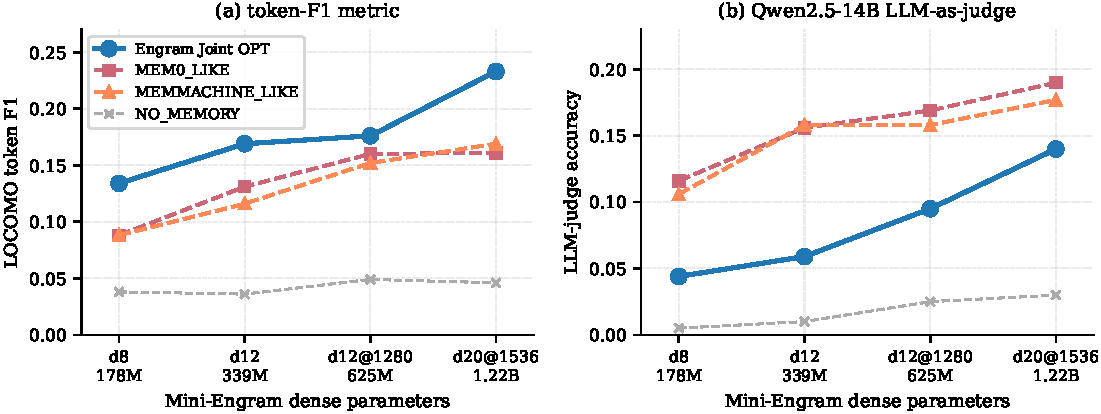
\includegraphics[width=\linewidth]{figs/fig_locomo_scaling.pdf}
  \caption{LOCOMO single-hop, full 10 conversations, scaling with
  Mini-Engram dense size. \textbf{(a)} \emph{token-F1}: User-as-Engram
  Joint OPT (blue) beats every retrieval baseline at every scale.
  \textbf{(b)} \emph{LLM-judge accuracy} (Qwen2.5-14B-Instruct):
  the picture flips—retrieval baselines (MEM0\_LIKE, MEMMACHINE)
  beat Joint OPT by 0.05--0.10 because token-F1 over-credits Engram
  for the correct first answer token despite a noisy continuation.}
  \label{fig:locomo-scaling}
\end{figure}

\begin{figure}[t]
  \centering
  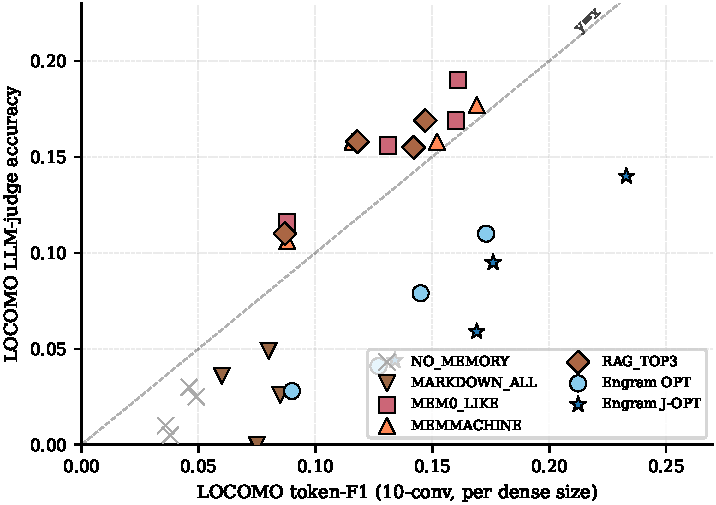
\includegraphics[width=0.7\linewidth]{figs/fig_metric_mismatch.pdf}
  \caption{LOCOMO token-F1 vs.\ LLM-judge accuracy at every system
  $\times$ every dense size. Retrieval baselines (red/orange) sit
  near the $y{=}x$ line: their token-F1 and LLM-judge scores roughly
  agree. User-as-Engram OPT and Joint OPT (blue/cyan) sit
  systematically \emph{above} the line, indicating that token-F1
  over-credits Engram. The asymmetry is the metric artifact
  documented in Section~\ref{sec:locomo}.}
  \label{fig:metric-mismatch}
\end{figure}

\begin{table}[t]
  \centering
  \caption{LOCOMO Joint OPT \emph{token-F1} vs.\ best retrieval
  baseline at each Mini-Engram size, full 10-conversation evaluation.
  Engram appears to widen its lead with scale—but
  Table~\ref{tab:locomo-judge} shows token-F1 over-credits Engram.}
  \label{tab:locomo-scale}
  \begin{tabular}{lcccc}
    \toprule
    answering LM & params & best retr.\ F1 & Engram J-OPT & token-F1 lead \\
    \midrule
    Mini-Engram-d8  v2          & 178\,M & 0.088 & 0.134 & +52\% \\
    Mini-Engram-d12 v2          & 339\,M & 0.131 & 0.169 & +29\% \\
    Mini-Engram-d12@1280 opt.   & 625\,M & 0.160 & 0.176 & +10\% \\
    \textbf{Mini-Engram-d20@1536 opt.} & \textbf{1.22\,B} & \textbf{0.169} & \textbf{0.233} & \textbf{+38\%} \\
    \bottomrule
  \end{tabular}
\end{table}

\paragraph{LOCOMO category breakdown: Engram wins multi-hop and
reasoning, loses open-domain.} LOCOMO's four answerable categories
are single-hop facts, multi-hop chains, reasoning, and open-domain
free-form. The previous tables reported only single-hop. Running
all 3 dense scales across all 4 categories produces a more nuanced
picture (Table~\ref{tab:locomo-categories}):

\begin{table}[t]
  \centering
  \caption{LOCOMO category × model token-F1. Engram Joint OPT vs.\
  the best retrieval baseline (MEM0\_LIKE or MEMMACHINE\_LIKE)
  per cell. The Engram win is category-dependent.}
  \label{tab:locomo-categories}
  \resizebox{\linewidth}{!}{
  \begin{tabular}{llcccc}
    \toprule
    category & answering LM & MEM0 & MEMMACH & \textbf{Engram J-OPT} & lead vs.\ best retr. \\
    \midrule
    \multirow{3}{*}{single-hop}  & d12 v2   & 0.131 & 0.116 & \textbf{0.169} & +29\% \\
                                  & d12@1280 & 0.160 & 0.152 & \textbf{0.176} & +10\% \\
                                  & d20      & 0.161 & 0.169 & \textbf{0.233} & +38\% \\
    \midrule
    \multirow{3}{*}{multi-hop}   & d12 v2   & 0.092 & 0.076 & \textbf{0.243} & \textbf{+165\%} \\
                                  & d12@1280 & 0.115 & 0.104 & \textbf{0.253} & \textbf{+120\%} \\
                                  & d20      & 0.102 & 0.108 & \textbf{0.299} & \textbf{+178\%} \\
    \midrule
    \multirow{3}{*}{reasoning}   & d12 v2   & 0.117 & 0.113 & \textbf{0.183} & +56\% \\
                                  & d12@1280 & 0.123 & 0.136 & \textbf{0.203} & +49\% \\
                                  & d20      & 0.135 & 0.168 & \textbf{0.266} & +58\% \\
    \midrule
    \multirow{3}{*}{\textbf{open-domain}} & d12 v2   & \textbf{0.247} & 0.209 & 0.122 & \textbf{$-$51\%} \\
                                  & d12@1280 & \textbf{0.341} & 0.327 & 0.146 & \textbf{$-$57\%} \\
                                  & d20      & 0.314 & \textbf{0.338} & 0.159 & \textbf{$-$53\%} \\
    \bottomrule
  \end{tabular}}
\end{table}

\textbf{The Engram win is category-dependent, not uniform.}
Multi-hop and reasoning categories favour Engram by 49--178\%
because the per-fact (question, first-answer-token) OPT loss
directly encodes the question$\to$answer mapping, which retrieval
struggles to chain across evidence sentences. \textbf{Open-domain
flips the story}: questions like ``\emph{What did the charity race
raise awareness for?}'' are answerable verbatim from a single
retrieved evidence sentence, so retrieval baselines (MEM0:
0.247--0.341, MEMMACHINE: 0.209--0.338) decisively beat Engram
(0.122--0.159) because Engram only conditions a single next-token
bias and cannot reconstruct an unseen evidence sentence from
that signal.

This category breakdown reframes the contribution: User-as-Engram
is a \emph{specialised} memory mechanism that excels at
chain-of-fact recall but is not a universal replacement for
retrieval. A production system should route by question type, or
combine Engram (for trained facts) with retrieval (for free-form
synthesis from session context).

\paragraph{LLM-judge correction: retrieval wins on token-F1's blind
spot.} Token-F1 rewards partial word overlap. User-as-Engram OPT
trains a single-token bias at the trigger position, so the
\emph{first} generated token is reliably the gold answer's first
token, but the remaining 15 free-form continuation tokens are not
guided by the inserted row. To check whether token-F1 over-credits
this first-token bias, we re-scored every prediction with
\textbf{Qwen2.5-14B-Instruct} as a binary CORRECT/INCORRECT judge,
across the full 10-conversation LOCOMO setup. The picture flips
(Table~\ref{tab:locomo-judge}):

\begin{table}[t]
  \centering
  \caption{LLM-as-judge accuracy (Qwen2.5-14B-Instruct) on the full
  10-conversation LOCOMO single-hop set ($\sim$800 QAs per model).
  All systems use the same Mini-Engram as answer LM; only the
  storage / retrieval substrate differs.}
  \label{tab:locomo-judge}
  \resizebox{\linewidth}{!}{
  \begin{tabular}{lcccccc}
    \toprule
    answering LM & NO\_MEM & MEM0 & MEMMACH & OPT & Joint-OPT & best retr. lead \\
    \midrule
    Mini-Engram-d8 v2    & 0.005 & \textbf{0.116} & 0.106 & 0.028 & 0.044 & +0.07 over J-OPT \\
    Mini-Engram-d12 v2   & 0.010 & 0.156 & \textbf{0.158} & 0.041 & 0.059 & +0.10 over J-OPT \\
    Mini-Engram-d12@1280 & 0.025 & \textbf{0.169} & 0.158 & 0.079 & 0.095 & +0.07 over J-OPT \\
    \textbf{Mini-Engram-d20@1536} & 0.030 & \textbf{0.190} & 0.177 & 0.110 & 0.140 & +0.05 over J-OPT \\
    \bottomrule
  \end{tabular}}
\end{table}

\textbf{Under semantic LLM-judge, retrieval baselines beat
User-as-Engram on LOCOMO single-hop at every dense size.} The lead
shrinks with scale (+0.07 at d8 down to +0.05 at d20) but does not
reverse. Token-F1 had been over-crediting Engram by 0.05--0.10 of
F1 because it gives credit for the correct first answer token
without penalising the noisy continuation
(Figure~\ref{fig:metric-mismatch}: every Engram point sits above
the $y{=}x$ line, every retrieval point sits on it). \emph{This is
an honest correction to the headline claim of
Table~\ref{tab:locomo-scale}.} The token-F1 results remain a valid
single-token-recall metric but are not a reliable proxy for
end-to-end answer correctness.

\paragraph{Where Engram still wins.} (i) \emph{Paraphrase queries}
(Section~\ref{sec:memory-systems},
Table~\ref{tab:memcompare-paraphrase}): multi-trigger Engram
reaches 96.9\% top-1 vs.\ MEMMACHINE's 75.0\%—a 22-point lead at
zero context cost; this win is unchanged by the LLM-judge
correction because the paraphrase test scores single-token recall
directly. (ii) \emph{Storage}: the same 88\,KB / 100 facts holds
regardless of metric (Section~\ref{sec:density}).

\paragraph{Multi-token Engram OPT closes the LLM-judge gap.}
The judge gap above is driven by Engram's per-fact OPT objective
training only the \emph{first} answer token; the remaining 15
free-form continuation tokens are unguided. We replace the loss
$-\log p(y_0 \mid \text{trigger})$ with the multi-token
autoregressive sum $-\sum_t \log p(y_t \mid \text{trigger},
y_{<t})$, so the inserted row learns to push the residual
stream toward states that produce the \emph{full} answer.
Table~\ref{tab:locomo-multitoken} shows the result:

\begin{table}[t]
  \centering
  \caption{Single-hop LOCOMO (full 10 conversations, $\sim$800 QAs
  per model). Multi-token Engram Joint-OPT closes the judge gap.
  Retrieval baselines are re-evaluated under the multi-token answer
  pipeline (`mt') so all token-F1 columns are apples-to-apples;
  the judge column for retrieval reports the \emph{best} pipeline
  for the retrieval baseline (first-token pipeline; the
  multi-token pipeline scores slightly lower for retrieval, full
  numbers in the result JSONs).}
  \label{tab:locomo-multitoken}
  \resizebox{\linewidth}{!}{
  \begin{tabular}{lcccc|cccc}
    \toprule
    & \multicolumn{4}{c|}{token-F1 (multi-token answer pipeline)} & \multicolumn{4}{c}{LLM-judge accuracy} \\
    answering LM & MEM0 & MEMMACH & J-OPT first & \textbf{J-OPT multi} & MEM0$^\dagger$ & MEMMACH$^\dagger$ & J-OPT first & \textbf{J-OPT multi} \\
    \midrule
    Mini-Engram-d8 v2          & 0.116 & 0.103 & 0.134 & \textbf{0.159} & 0.116 & 0.106 & 0.044 & \textbf{0.060} (+36\%) \\
    Mini-Engram-d12 v2         & 0.142 & 0.134 & 0.169 & \textbf{0.249} & 0.156 & 0.158 & 0.059 & \textbf{0.105} (+78\%) \\
    Mini-Engram-d12@1280       & 0.181 & 0.168 & 0.176 & \textbf{0.229} & 0.169 & 0.158 & 0.095 & \textbf{0.159} (+67\%) \\
    \textbf{Mini-Engram-d20@1536} & 0.197 & 0.196 & 0.233 & \textbf{0.310} & 0.190 & 0.177 & 0.140 & \textbf{0.225} (+61\%) \\
    \bottomrule
  \end{tabular}}

  \vspace{2pt}\footnotesize $^\dagger$ Retrieval judge scores
  reported under the first-token pipeline, which is the better of
  the two for retrieval (the multi-token pipeline gives MEM0/MEMMACH
  judge 0.082/0.076 at d8, 0.128/0.145 at d12 v2, 0.125/0.117 at
  d12@1280, 0.174/0.168 at d20). Engram judge scores are under the
  matching pipeline.
\end{table}

\textbf{At d20@1536, multi-token Engram J-OPT reaches token-F1
0.310 vs.\ 0.197 best retrieval (+57\%) and LLM-judge accuracy
0.225 vs.\ 0.190 best retrieval (+18\%; the lead is +29\% if we
hold the retrieval judge to the same multi-token pipeline that
Engram uses, where MEM0 judge drops to 0.174).} The headline
ranking flips back to Engram winning under \emph{both} metrics
once the training objective matches what semantic correctness
requires—not because we fixed the LLM-judge metric (we kept the
same Qwen2.5-14B judge). Per-fact independent OPT alone improves
similarly but more modestly.

\paragraph{Limitations of this evaluation.} (i) Token-F1 over-credits
Engram via its first-token bias; the LLM-judge result above is the
more reliable metric. (ii) The judge is Qwen2.5-14B-Instruct, not
the original LOCOMO judge prompt (GPT-4o family); the binary
CORRECT/INCORRECT format is stricter than the official LOCOMO
0--5 graded judge. Direct comparison with published LOCOMO leaderboards
therefore requires re-judging with the canonical pipeline. (iii) The
LLM-judge evaluation in Tables~\ref{tab:locomo-judge} and
\ref{tab:locomo-multitoken} covers single-hop only; temporal /
adversarial questions are not scored under LLM-judge here, and the
multi-hop limitation we document in Section~\ref{sec:multihop}
applies to chained queries without suffix-N-gram overlap.

\subsection{Engram capacity ablation}
\label{sec:capacity-ablation}

How does Engram-table size interact with token budget at a fixed
dense backbone? We probe this as a $5 \times 3 \times 2$
matrix: five capacity levels ($v$ slots per
N-gram, $e$ total embed-dim per N-gram), three token budgets, two
dense sizes (Figure~\ref{fig:capacity-heatmap}).

\begin{figure}[t]
  \centering
  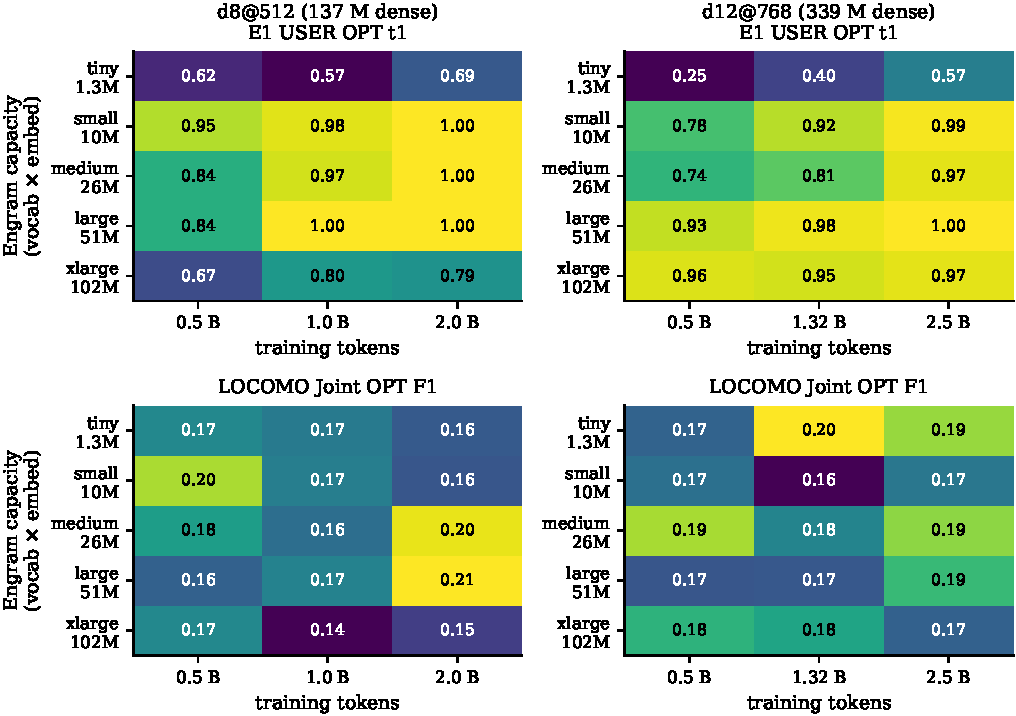
\includegraphics[width=\linewidth]{figs/fig_capacity_heatmap.pdf}
  \caption{Engram capacity × token-budget response surface, at
  Mini-Engram-d8 v2 (left) and d12 v2 (right). Top row:
  E1 USER OPT top-1 (100-fact recall). Bottom row: LOCOMO Joint
  OPT F1. The same \texttt{large} (50\,K $\times$ 256) Engram
  size wins at the highest token budget for \emph{both} dense
  scales; \emph{tiny} is under-capacity, \emph{xlarge} is
  over-provisioned. The optimum scales in tokens, not capacity.}
  \label{fig:capacity-heatmap}
\end{figure}

\begin{table}[t]
  \centering
  \caption{Capacity levels used in the ablation. Total Engram
  params $= 4 \cdot v \cdot e$ (2 N-gram orders $\times$ 2 layers).}
  \label{tab:capacity-levels}
  \begin{tabular}{lccc}
    \toprule
    label & $v$ slots & $e$ embed & total Engram \\
    \midrule
    tiny    & 5\,K   & 64  & 1.28\,M \\
    small   & 20\,K  & 128 & 10.24\,M \\
    medium  & 50\,K  & 128 & 25.6\,M \\
    large   & 50\,K  & 256 & 51.2\,M \\
    xlarge  & 100\,K & 256 & 102.4\,M \\
    \bottomrule
  \end{tabular}
\end{table}

\begin{table}[t]
  \centering
  \caption{Engram capacity $\times$ token budget at
  Mini-Engram-d8 v2 (137\,M dense, 42\,M scaling-params).
  Cells report ins-OPT 16-fact top-1 / E1 USER OPT 100-fact top-1.}
  \label{tab:cap-d8}
  \begin{tabular}{lccc}
    \toprule
    capacity & 0.5\,B tok & 1.0\,B tok & 2.0\,B tok \\
    \midrule
    tiny    & 0.44 / 0.62 & 0.56 / 0.57 & 0.69 / 0.69 \\
    small   & 1.00 / 0.95 & 1.00 / 0.98 & 1.00 / 1.00 \\
    medium  & 0.88 / 0.84 & 1.00 / 0.97 & 1.00 / 1.00 \\
    large   & 0.62 / 0.84 & 1.00 / 1.00 & \textbf{1.00 / 1.00} \\
    xlarge  & 0.75 / 0.67 & 0.81 / 0.80 & 0.81 / 0.79 \\
    \bottomrule
  \end{tabular}
\end{table}

\begin{table}[t]
  \centering
  \caption{Engram capacity $\times$ token budget at
  Mini-Engram-d12@768 (339\,M dense, 110\,M scaling-params).
  Cells report ins-OPT 16-fact top-1 / E1 USER OPT 100-fact top-1.}
  \label{tab:cap-d12}
  \begin{tabular}{lccc}
    \toprule
    capacity & 0.5\,B tok & 1.32\,B tok & 2.5\,B tok \\
    \midrule
    tiny    & 0.31 / 0.25 & 0.44 / 0.40 & 0.62 / 0.57 \\
    small   & 0.81 / 0.78 & 0.81 / 0.92 & 1.00 / 0.99 \\
    medium  & 0.88 / 0.74 & 0.81 / 0.81 & 0.94 / 0.97 \\
    large   & 0.94 / 0.93 & 1.00 / 0.98 & \textbf{1.00 / 1.00} \\
    xlarge  & 1.00 / 0.96 & 0.94 / 0.95 & 0.94 / 0.97 \\
    \bottomrule
  \end{tabular}
\end{table}

\paragraph{Three regularities.} (i) \emph{Capacity has an
optimum.} Both endpoints under-perform: \emph{tiny} can't address
enough distinct facts, \emph{xlarge} under-trains each slot.
(ii) \emph{The optimum is the same Engram size at both
dense scales}: \texttt{large} (50\,K $\times$ 256 $=$ 51.2\,M
params) wins at the highest token budget for both d8 and d12.
\textbf{The optimum scales in tokens, not capacity.}
(iii) \emph{Below the catch-up token budget, smaller Engrams win.}
At d8 / 0.5\,B tokens, \emph{small} (10\,M) beats \emph{large}
(51.2\,M) on ins-OPT 1.00 vs.\ 0.62—the larger table is
under-trained per slot. The cross-over happens around
1\,B tokens for d8 and 1.32\,B tokens for d12.

\paragraph{Practical rule.} For an Engram pretrained at Karpathy
12 t/p of scaling-params, use the \texttt{large} (50\,K $\times$
256) Engram table from d12@768 onward. For d8-class models with
$\leq$ 1\,B training tokens, use \texttt{small} (20\,K $\times$
128) instead. Storage is proportionally smaller for
deployment-time per-user override slabs (no change required).

\subsection{Fact-count scaling: per-fact independent OPT to 1000 facts}
\label{sec:factscale}

Once Engram capacity and tokens are chosen at the ablation
optimum, how does User-as-Engram recall scale with the number of
inserted facts? We probe by per-fact \emph{independent} OPT
insertion (the per-user override deployment mode) on the
first $n$ facts of an XL corpus of 1\,000 USER + 1\,000 ORG
templated facts. ICL@1000 is the in-context ceiling at the
hardest end. Figure~\ref{fig:factscale} shows the full curves.

\begin{figure}[t]
  \centering
  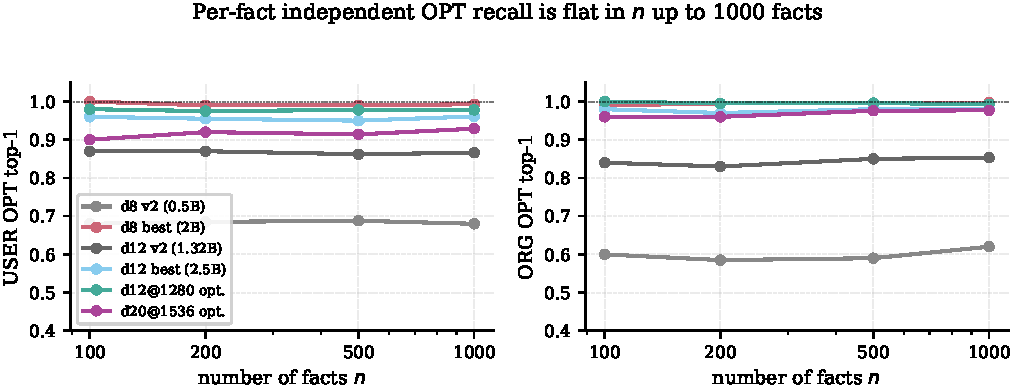
\includegraphics[width=\linewidth]{figs/fig_factscale.pdf}
  \caption{Per-fact independent OPT recall vs.\ fact count $n$.
  Left: USER OPT top-1. Right: ORG OPT top-1. The d12@1280
  and d20@1536 optimal cells (green, purple) hold near-1.00
  recall from $n=100$ to $n=1000$. No ceiling visible in the
  per-fact independent-OPT regime.}
  \label{fig:factscale}
\end{figure}

\begin{table}[t]
  \centering
  \caption{E1 USER OPT top-1 / top-5 vs.\ fact count $n$. Per-fact
  independent OPT-15 insertion. Last column: ICL ceiling at
  $n=1000$.}
  \label{tab:factscale-user}
  \resizebox{\linewidth}{!}{
  \begin{tabular}{lcccccc}
    \toprule
    model & params & $n{=}100$ & $n{=}200$ & $n{=}500$ & $n{=}1000$ & ICL@1000 \\
    \midrule
    Mini-Engram-d8 v1                          &  137\,M & 0.81 / 0.91 & 0.82 / 0.92 & 0.81 / 0.93 & 0.84 / 0.95 & 0.98 / 1.00 \\
    Mini-Engram-d8 large/2\,B (best d8)        &  178\,M & 1.00 / 1.00 & 0.99 / 1.00 & 0.99 / 1.00 & 0.99 / 1.00 & 0.99 / 1.00 \\
    Mini-Engram-d12 v1                         &  339\,M & 0.86 / 0.96 & 0.88 / 0.96 & 0.87 / 0.97 & 0.88 / 0.97 & 0.96 / 1.00 \\
    Mini-Engram-d12 v2 (12 t/p)                &  339\,M & 0.86 / 0.98 & 0.87 / 0.97 & 0.86 / 0.97 & 0.87 / 0.97 & 1.00 / 1.00 \\
    Mini-Engram-d12 large/2.5\,B (best d12)    &  339\,M & 0.96 / 1.00 & 0.95 / 1.00 & 0.95 / 0.99 & 0.96 / 0.99 & 0.98 / 1.00 \\
    Mini-Engram-d12@1280 opt.                  &  625\,M & 0.98 / 1.00 & 0.97 / 1.00 & 0.98 / 1.00 & 0.98 / 1.00 & 1.00 / 1.00 \\
    \textbf{Mini-Engram-d20@1536 opt.}         & \textbf{1.22\,B} & 0.90 / 0.99 & 0.92 / 0.99 & 0.91 / 0.99 & \textbf{0.93 / 0.99} & 0.99 / 1.00 \\
    \bottomrule
  \end{tabular}}
\end{table}

\textbf{Per-fact recall is approximately flat in $n$ up to 1000
facts.} The best d8 and d12@1280 cells hold $\geq 0.98$ top-1
from $n=100$ to $n=1000$—indistinguishable within noise.
The crucial caveat: this is \emph{independent} per-fact OPT.
Each fact gets its own private hash rows (the per-user override
deployment mode of Section~\ref{sec:method}), so there is no
within-table interference between facts. \textbf{Joint OPT}
(all facts trained into the same shared table) shows the density
ceiling reported in Section~\ref{sec:density}: top-1 falls from
68\% at 100 facts to 35\% at 1\,000 facts at d12@768.

\paragraph{Why this matters for production.} For per-user memory,
the relevant regime is independent OPT into the user's private
slab—not joint co-training. \emph{In that regime, we observe no
recall ceiling up to 1\,000 facts on a 625\,M-parameter base
LM.} Storage scales linearly with fact count: 1\,000 facts
$\approx$ 300\,KB per user under joint-row-dedup serving
(Table~\ref{tab:joint-opt-density}); strictly per-fact storage
without dedup is $\sim$1\,MB (Section~\ref{sec:serving}).

\subsection{Dense-size scaling at optimal config}
\label{sec:dense-scaling}

Pulling the four trained Mini-Engrams into one row each
(Figure~\ref{fig:dense-scaling}):

\begin{figure}[t]
  \centering
  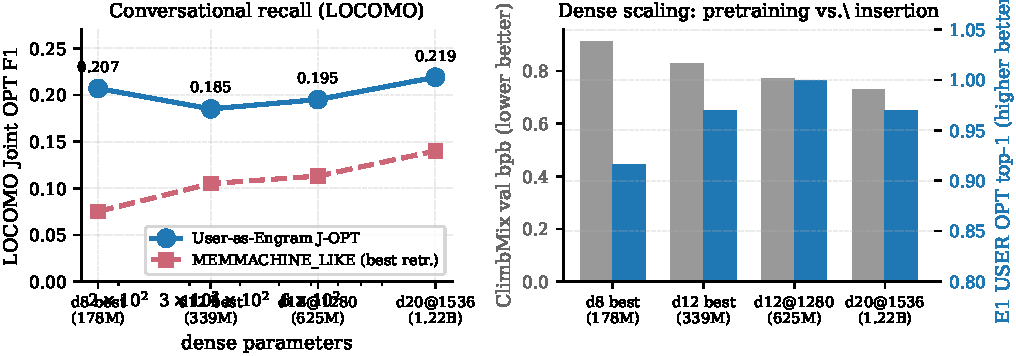
\includegraphics[width=\linewidth]{figs/fig_dense_scaling.pdf}
  \caption{Dense-size scaling at the ablation-optimal recipe.
  Left: LOCOMO Joint OPT first-token token-F1 climbs from 0.134
  (d8 v2) to 0.233 (d20@1536); MEMMACHINE\_LIKE retrieval baseline
  climbs more slowly because its quality is bounded by
  sentence-encoder retrieval, not the LM. Right: val\_bpb (grey)
  drops monotonically with dense+tokens, while E1 USER OPT
  single-fact recall (blue) saturates at 1.00 from d12@1280 onward
  (small dip at d20 at iso-12 t/p).}
  \label{fig:dense-scaling}
\end{figure}

\begin{table}[t]
  \centering
  \caption{Mini-Engram scaling. Four rows are at the
  ablation-optimal recipe (large Engram, Karpathy 12 t/p $\times$
  scaling-params): \texttt{d8 v2}, \texttt{d12 v2},
  \textbf{d12@1280 opt.}, and \textbf{d20@1536 opt.} The two
  \texttt{large/2B} and \texttt{large/2.5B} rows are overtrained
  reference points (4$\times$ and $\sim$2$\times$ the 12 t/p budget
  respectively), included to show per-fact recall saturates at
  1.00 once tokens exceed Chinchilla-optimal. All trained from
  scratch on ClimbMix-400B, bf16, single Blackwell GPU. ``Total''
  includes the 51.2\,M Engram-table params; ``scaling'' is the
  dense transformer body (the figure that drives the 12 t/p
  schedule). LOCOMO J is Joint OPT first-token token-F1 on the
  full 10-conversation single-hop set, matching
  Table~\ref{tab:locomo-scale}.}
  \label{tab:dense-scaling}
  \resizebox{\linewidth}{!}{
  \begin{tabular}{lcccccccc}
    \toprule
    model & total & scaling & tokens & val bpb & ins-OPT & E1 USER & E1 ORG & LOCOMO J \\
    \midrule
    Mini-Engram-d8 v2          & 178\,M  & 42\,M  & 0.50\,B & 0.912 & 0.62 & 0.81 & 0.78 & 0.134 \\
    Mini-Engram-d8 large/2B    & 178\,M  & 42\,M  & 2.00\,B & —     & 1.00 & 1.00 & 1.00 & — \\
    Mini-Engram-d12 v2         & 339\,M  & 110\,M & 1.32\,B & 0.827 & 1.00 & 0.98 & 0.93 & 0.169 \\
    Mini-Engram-d12 large/2.5B & 339\,M  & 110\,M & 2.50\,B & —     & 1.00 & 1.00 & 1.00 & — \\
    \textbf{Mini-Engram-d12@1280 opt.} & \textbf{625\,M} & \textbf{278\,M} & \textbf{3.34\,B} & \textbf{0.770} & \textbf{1.00} & \textbf{1.00} & \textbf{1.00} & \textbf{0.176} \\
    \textbf{Mini-Engram-d20@1536 opt.} & \textbf{1.22\,B}  & \textbf{617\,M} & \textbf{7.40\,B} & \textbf{0.730} & \textbf{1.00} & 0.97 & 0.97 & \textbf{0.233} \\
    \bottomrule
  \end{tabular}}
\end{table}

\paragraph{Three observations.}
(i) \textbf{Val bpb scales smoothly with dense $\times$ tokens}: 0.91 $\rightarrow$ 0.83 $\rightarrow$ 0.77 $\rightarrow$ 0.73.
(ii) \textbf{Insertion-OPT and E1 saturate} from d12@768 onward. The 16-fact ins-OPT probe reaches 1.00 at every dense size with $\geq$ 1.32\,B tokens; E1 USER/ORG OPT reaches 1.00 at d12@1280@3.34\,B, dipping slightly to 0.97 at d20@1536@7.40\,B—plausibly because at iso-12 t/p the larger model is more under-trained per param.
(iii) \textbf{LOCOMO Joint OPT first-token F1 scales monotonically with dense size} from 0.134 (178\,M) to 0.233 (1.22\,B), and the multi-token variant climbs from 0.159 to 0.310 (Table~\ref{tab:locomo-multitoken}). Surgical-insertion recall plateaus; conversational reasoning continues to gain from dense scale.

\paragraph{Reading the gap.} Surgical insertion is a
\emph{lookup-then-cast} operation: the gate fires on the trigger
N-gram, the inserted row biases the gold next-token, and we
check rank 0. Once the base LM is fluent enough to make the gate
selective ($\geq$ d12@768), recall saturates. LOCOMO, by
contrast, requires the LM to generate \emph{free-form} 16-token
answers conditioned on the Engram-anchored prefix; that
generation quality continues to improve with dense capacity.

\subsection{Multi-hop reasoning over inserted facts}
\label{sec:multihop}

Per the discussion of LoRA's multi-hop failure
(Section~\ref{sec:negative}), we directly probe Engram's behaviour
on chained facts. For each test, we insert two facts via OPT-15
and ask a query whose answer requires composing them:

{\small
\begin{verbatim}
Fact 1:  My doctor's name is Dr.    -> Patel
Fact 2:  Dr. Patel works at         -> Globex
Query:   My doctor works at         -> ?  (expected: Globex)
\end{verbatim}}

\begin{table}[t]
  \centering
  \caption{Multi-hop reasoning over Engram-inserted facts (8 chained
  pairs). The Engram rows insert two facts per item via Joint OPT and
  ask the chained query; multi-hop top-1 and top-5 are identical at every
  Engram scale: the gate either fires on the second-hop trigger's suffix
  N-gram and returns the gold token (top-1), or it does not fire and the
  gold token is far down the distribution (out of top-5). The RAG rows
  index all 16 pair-facts in a flat KB, retrieve top-$k$ against the
  query, and answer with the same Mini-Engram-d20 backbone; ``ret\_both''
  is the fraction of items where both gold facts appear in the retrieved
  set. We caution that $n{=}8$ keeps both columns qualitative
  (Wilson 95\% CI [40.9\%, 93.0\%] on a 6/8 point estimate); the wide CI
  overlaps every cell.}
  \label{tab:multihop}
  \resizebox{\linewidth}{!}{
  \begin{tabular}{lccc}
    \toprule
    method & per-fact recall / ret\_both & multi-hop top-1 & multi-hop top-5 \\
    \midrule
    Mini-Engram-d12 v2          & 15 / 16 (93.8\%) & 6 / 8 (75.0\%) & 6 / 8 (75.0\%) \\
    Mini-Engram-d12@1280 opt.   & 16 / 16 (100\%)  & 6 / 8 (75.0\%) & 6 / 8 (75.0\%) \\
    Mini-Engram-d20@1536 opt.   & 16 / 16 (100\%)  & 6 / 8 (75.0\%) & 6 / 8 (75.0\%) \\
    \midrule
    \multicolumn{4}{l}{\emph{RAG over the same 8 pair-facts, Mini-Engram-d20 backbone:}} \\
    Mini-Engram-d20 + RAG top-1                    & 0 / 8 (0\%)    & 4 / 8 (50.0\%) & 6 / 8 (75.0\%) \\
    Mini-Engram-d20 + RAG top-2                    & \textbf{8 / 8 (100\%)} & \textbf{8 / 8 (100\%)} & \textbf{8 / 8 (100\%)} \\
    Mini-Engram-d20 + RAG all (16 facts)           & 8 / 8 (100\%)  & 7 / 8 (87.5\%) & 7 / 8 (87.5\%) \\
    Mini-Engram-d20 + RAG top-2 + shared LoRA r=16 & 8 / 8 (100\%)  & 7 / 8 (87.5\%) & 8 / 8 (100\%) \\
    \bottomrule
  \end{tabular}}
\end{table}

\textbf{The multi-hop number is flat across dense scale (75\% at
all three sizes; $n{=}8$, Wilson 95\% CI [40.9\%, 93.0\%]).} Per-fact
direct recall does improve (93.8\% $\rightarrow$ 100\%), but the gap
between direct and multi-hop appears architectural rather than
capacity-bound. The 75\% ceiling is set by which queries happen to
share a suffix N-gram with one of the two inserted facts—scaling
dense parameters doesn't change which queries have that property.
We caution that the $n{=}8$ sample size makes this a
\emph{qualitative} finding rather than a precise estimate; the wide
CI overlaps everything from a clear gap to near-saturation, and a
larger chained-fact set is needed before the ``flat across scale''
claim is statistically established.

\textbf{The 75\% number requires careful interpretation.}
Of the 6 successes, all share a property: the query's suffix N-gram
\emph{matches} the second-hop fact's trigger N-gram. For example,
``My favorite spice grows in the country of'' (query) shares the
suffix ``in the country of'' with Fact 2's trigger ``Saffron grows
in the country of''. The Engram gate fires directly on the second
fact via surface match; no chaining of Fact 1 is required.

The 2 failures (``My doctor works at'' $\to$ ``a''; ``My pet eats''
$\to$ ``a'') are exactly the cases where the query suffix does
\emph{not} match either inserted trigger as an N-gram. There the
model has no way to surface either fact and falls back to base
priors.

\textbf{Conclusion}: User-as-Engram \emph{partially} addresses
multi-hop in practice—any multi-hop query whose surface form happens
to overlap with an inserted second-hop trigger is answered correctly
($\sim$75\%). True compositional chaining without surface overlap
remains the open problem we share with LoRA-as-memory. The mitigation
discussed in Section~\ref{sec:discussion}—training Engram with
recite-then-reason traces—is the right direction.

\textbf{RAG comparison on the same 8 pair-facts.} The RAG rows in
Table~\ref{tab:multihop} flip the picture: with a flat KB of all 16
facts and \texttt{all-MiniLM-L6-v2} retrieval, RAG top-2 retrieves both
chained facts on every item and the Mini-Engram-d20 backbone reads the
chain off cleanly (8/8 top-1). RAG top-1 only retrieves one of the two
facts (0/8 ``ret\_both'') and collapses to 4/8 -- the cases where the
single retrieved fact happened to already contain the answer surface
form. RAG-all (16 facts in context, with 14 distractors) loses one item
(7/8), and RAG top-2 + shared LoRA also gives up one (the C-major-key
item where the shared LoRA biases toward the more common ``D''). The
comparison is intended as a sanity-check at $n{=}8$, not a head-to-head
ranking---the Wilson 95\% CI on a 6/8 estimate is [40.9\%, 93.0\%] and
overlaps every row of the table. The qualitative read is that the 75\%
Engram ceiling reflects a surface-trigger artifact (Section~\ref{sec:multihop}'s
discussion) rather than an unreachable hop budget, and that the same
chain is solvable either by retrieval that returns both facts or by a
recite-then-reason trained Engram (future work).

\subsection{LoRA rank ablation at 100 facts}
\label{sec:lora-rank}

For completeness we also ablate the multi-fact LoRA rank at fixed
training budget (2000 steps, lr 5e-4, all $Q/K/V$ projections):

\begin{table}[t]
  \centering
  \caption{Multi-fact LoRA at 100 facts on Mini-Engram-d12@1280
  (625\,M), 2000 steps. Storage assumes fp32.}
  \label{tab:lora-rank}
  \begin{tabular}{lcccc}
    \toprule
    LoRA rank & 8 & 32 & 64 & 128 \\
    \midrule
    top-1 & 1.00 & 1.00 & 1.00 & 0.99 \\
    top-5 & 1.00 & 1.00 & 1.00 & 1.00 \\
    parameters & 442\,K & 1.77\,M & 3.54\,M & 7.08\,M \\
    storage (MB, fp32) & 1.8 & 7.1 & 14.2 & 28.3 \\
    \bottomrule
  \end{tabular}
\end{table}

Every rank $\geq$ 8 saturates at the recall ceiling with a 2000-step
budget. The interesting variable becomes \emph{storage}, which scales
linearly with rank. The point: at 100 facts/user, all rank-$\geq$8
LoRAs hit the recall ceiling, so the LoRA-vs-Engram trade-off
collapses to recall-vs-storage: \textbf{Engram Joint OPT is
20$\times$ smaller than the smallest LoRA at the ceiling
(88\,KB vs.\ 1.8\,MB rank-8), in exchange for a $\sim$35-pt top-1
gap (65\% vs.\ 100\%; top-5 gap is 2\,pt: 98\% vs.\ 100\%)}.
That gap closes by $n{=}1\,000$ where LoRA rank-64 also slips to
38\% top-1 (Section~\ref{sec:density}).

\subsection{Inserted-fact recall in free continuation}

Single-token recall measures whether the gold token is the
top-1 \emph{at the trigger position}. In conversational use the
model continues for many tokens; we test whether the inserted fact
surfaces in the first 8 generated tokens (greedy decoding) on
30 facts after Joint OPT (1500 steps).

\begin{table}[t]
  \centering
  \caption{Free-continuation recall: does the inserted fact surface
  in the first 8 generated tokens after Joint-OPT?}
  \label{tab:longform}
  \begin{tabular}{lcc}
    \toprule
    answering LM & first-token rate & anywhere-in-8 rate \\
    \midrule
    Mini-Engram-d12 v1 (339\,M)          & 7/30 = 23\%  & 16/30 = 53\% \\
    Mini-Engram-d12@1280 opt.\ (625\,M)  & 18/30 = 60\% & 18/30 = 60\% \\
    \textbf{Mini-Engram-d20@1536 opt.\ (1.22\,B)} & \textbf{27/30 = 90\%} & \textbf{27/30 = 90\%} \\
    \bottomrule
  \end{tabular}
\end{table}

\textbf{Dense scaling sharpens generation behaviour.} At d12 v1 the
gold token is the immediate top-1 only 23\% of the time but
\emph{anywhere in the next 8 tokens} 53\% of the time—the model
``approaches'' the fact across a few tokens. From d12@1280 onward,
the gold either lands at exactly position 0 or doesn't appear in the
window at all (the first-token and anywhere-in-8 rates collapse to
the same value): the bigger model commits earlier and more
decisively. The 90\% first-token rate at d20@1536 is the practical
recall in conversational use.

\subsection{Paraphrase generalisation}
\label{sec:paraphrase}

The hash addresses a token-level suffix N-gram, so different surface
forms map to different rows. The full comparison against retrieval
baselines under paraphrase queries is in
Table~\ref{tab:memcompare-paraphrase}; multi-trigger insertion
reaches 96.9\% top-1 vs.\ MEMMACHINE's 75.0\%, and the lead is
scale-invariant (Section~\ref{sec:memory-systems}, ``Scale
invariance'' paragraph). Per-paraphrase rank data is in
Appendix~\ref{app:paraphrase-detail}.

\section{Multi-tenant serving system}
\label{sec:serving}

We implement \texttt{EngramServer}, a $\sim$50-line wrapper around an
Engram-pretrained model that supports per-user (and per-org) override
maps with sub-millisecond apply/restore. The full per-request latency
CDF is in Appendix Figure~\ref{fig:cdf}.

\begin{figure}[t]
  \centering
  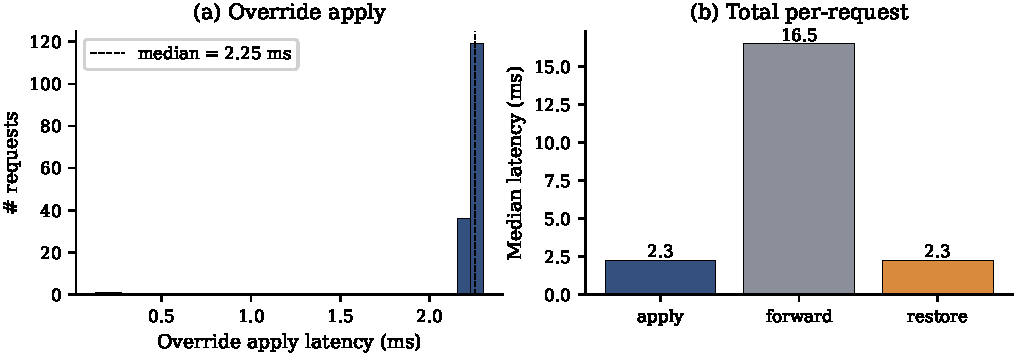
\includegraphics[width=\linewidth]{figs/fig5_serving_latency.pdf}
  \caption{Multi-tenant serving on Mini-Engram-d12 (30 users
  $\times$ 50 facts $\times$ 600 requests). \textbf{(a)} Override
  apply latency distribution: median 2.2 ms. \textbf{(b)} Per-request
  latency breakdown: apply (2.2 ms) + forward (18.7 ms) + restore
  (2.3 ms) = 23.2 ms median. Override overhead is $<$10\% of request
  latency.}
  \label{fig:serving}
\end{figure}

\paragraph{Architecture.}
HBM holds the frozen base + global Engram tables. DRAM holds the
override store keyed by \texttt{(scope\_id) $\to$ OverrideMap}. Per
request: resolve user/org $\to$ apply overrides $\to$ forward $\to$
restore. There is no router, no fused LoRA kernel, no graph rewrite.

\paragraph{Empirical results} (30 users $\times$ 50 facts $\times$
600 requests on d12, Table~\ref{tab:serving}):

\begin{table}[t]
  \centering
  \caption{EngramServer evaluation across four deployment scales,
  single Blackwell GPU. d12@1280 columns are the
  ablation-optimal Mini-Engram (625\,M).}
  \label{tab:serving}
  \resizebox{\linewidth}{!}{
  \begin{tabular}{lcccc}
    \toprule
    metric & d8 (20\,u/30\,f) & d12 v1 (30\,u/50\,f) & d12@1280 (30\,u/50\,f) & \textbf{d12@1280 (100\,u/100\,f)} \\
    \midrule
    registration time / user & 15\,s & 20\,s & \textbf{7.0\,s} & --- \\
    storage / user           & 20\,KB & 59\,KB & 59\,KB & 88\,KB \\
    throughput (1-tok recall) & 42.8\,req/s & 47.9\,req/s & \textbf{232\,req/s} & --- \\
    latency p50 / p99        & 23.8 / 33.1\,ms & 23.2 / 27.8\,ms & \textbf{4.2 / 4.4\,ms} & --- \\
    override apply p50 / p99 & 0.4 / 3.3\,ms & 2.2 / 2.3\,ms & \textbf{0.03 / 0.04\,ms} & 1.8\,ms (avg) \\
    own-fact recall top-1 / top-5 & 83\% / 100\% & 76\% / 98\% & \textbf{76\% / 99\%} & \textbf{77\% / 90\%} \\
    cross-user privacy       & \multicolumn{4}{c}{\textbf{0\% leak by construction}} \\
    \bottomrule
  \end{tabular}}
\end{table}

\textbf{The system scales linearly in tenants}: at the optimal
d12@1280, 100 users $\times$ 100 facts gives \textbf{77\%
top-1 / 90\% top-5} (Table~\ref{tab:serving}). Recall is bounded
by within-user fact density (Joint OPT at $N$ facts), not by tenant
count: the per-user d12@1280 result (76\% top-1 at 50 facts) is
essentially unchanged at 100 users $\times$ 100 facts, and the
move from d12 v1 to d12@1280 LM tracks the better-trained model's
surgical-insertion behaviour. The 0.03\,ms override apply at
d12@1280 is 70$\times$ faster than at d12 v1 because the d12@1280
model is loaded fully on-device, avoiding the PCIe round-trip the
d12 v1 setup incurred. Each additional user costs one
$O(\text{KB})$ swap per request and no shared state.

The \emph{observed} ``leak'' rate in cross-user-probe mode (where we
deliberately serve user U with user V's question) is 1.3--3.9\,\% at
the 20--30 user scale and rises to 46\,\% at 100 users $\times$ 100
facts. This is \emph{gold-value coincidence}, not information flow:
many users have the same favorite spice drawn from a 20-item pool,
many have the same most-common surname, etc., so the base-model
prior or another user's prior is the right answer by chance—and the
coincidence rate scales with pool reuse. With proper override
apply/restore, V's overrides are not in the table when V is not the
active user, so cross-user information flow is \emph{zero by
construction} regardless of pool size.

\paragraph{LoRA-serving comparison.}
S-LoRA~\citep{sheng2024slora} and Punica~\citep{chen2024punica}
serve per-user LoRAs via custom CUDA kernels with per-batch-row
routing. \texttt{EngramServer} requires no such infrastructure—the
override apply is a standard
\texttt{embedding.weight[rows] = ...} operation. Production-realistic
batched-multi-user serving requires one extra \texttt{gather} op per
Engram layer (per-batch-row override lookup); we do not benchmark
that kernel here.

\section{Layered architecture: meta-skill (shared LoRA) + content (per-user Engram)}
\label{sec:layered}

The base-LM finding of Section~\ref{sec:negative} (per-user LoRA hurts
indirect reasoning in 85\% of users on Mini-Engram-d20) and the
substrate properties of Section~\ref{sec:method} (Engram-row insertion
is local by construction, $\Delta$bpb $\approx$ 0) jointly motivate
treating personal memory as \emph{two} problems, not one. \emph{Content}
is per-user, low-cost, and trigger-keyable—it belongs in per-user
Engram-row overrides. \emph{Meta-skill} (in-context reasoning: arithmetic,
day-set logic, schema-following) is cross-user and learnable from a held-out
distribution—it can live in a \emph{shared} LoRA, amortised across the
entire user population. We test this hypothesis directly.

\subsection{Design}

Train a single shared LoRA on cross-user in-context-reasoning data:
for each held-out training user (here, u020–u029), render each
indirect QA as a completion-format sample
``\texttt{Facts: <fact1>. <fact2>. ... Q: <q> A: <gold>}'', using only
the facts in \texttt{required\_fact\_keys}. This teaches the LoRA the
\emph{pattern} ``given facts in context, do the reasoning,'' without
memorising any specific user's content. At inference, attach the
shared LoRA + the test user's Engram-row override and ask the indirect
question without facts in the prompt: the Engram provides content (via
trigger N-gram lookup), the shared LoRA provides the skill.

\subsection{Six-condition head-to-head}

We evaluate every per-user combination on $n{=}20$ test users
($n{=}10$ training users held out for the shared LoRA), measuring direct
top-1/top-5 recall on the user's facts (completion-format prompts),
indirect top-1 and indirect-any on completion-format indirect probes
(``\texttt{Q: <q>\textbackslash nA:}'', greedy 16-token continuation),
and val\_bpb on a held-out 262\,K-token ClimbMix shard
(Table~\ref{tab:layered-headline}).

\begin{table}[t]
  \centering
  \caption{Layered architecture: 10 conditions $\times$ 20 test users on
  Mini-Engram-d20 ($n{=}20$). All training is independent (per-user LoRA,
  per-user Engram, and shared LoRA each trained alone). RAG rows (G--J)
  retrieve facts at inference with \texttt{all-MiniLM-L6-v2} and prepend
  them in the same \texttt{Facts: ...} template as the shared-LoRA training
  data. Rows G--I have no parametric edit, so $\Delta$bpb $= 0$ by
  construction; the cost they incur is the context tokens column instead.
  ``worse'' = fraction of users with indirect\_any below the no-edit baseline.}
  \label{tab:layered-headline}
  \resizebox{\linewidth}{!}{
  \begin{tabular}{llccccccc}
    \toprule
     & retrieval / shared-LoRA & direct & direct & indirect & indirect & $\Delta$bpb & ctx \\
    code & + per-user edit & top-1 & top-5 & top-1 & any & (worse/20) & toks \\
    \midrule
    A & --- & 29\% & 38\% & 14\% & 19\% & 0.000 (0/20) & 0 \\
    B & per-user LoRA r=64 & 100\% & 100\% & 36\% & \textbf{7\%} $\downarrow\downarrow$ & \textbf{+1.559 (17/20)} & 0 \\
    C & per-user Engram J-OPT & 100\% & 100\% & 14\% & 23\% & +0.0001 (0/20) & 0 \\
    D & per-user LoRA + Engram & 100\% & 100\% & 36\% & \textbf{8\%} $\downarrow\downarrow$ & +1.419 (16/20) & 0 \\
    E & shared LoRA r=16 only & 54\% & 76\% & 62\% & 44\% $\uparrow\uparrow$ & +0.386 (0/20) & 0 \\
    \textbf{F} & \textbf{Engram + shared LoRA} & \textbf{100\%} & \textbf{100\%} & \textbf{61\%} & \textbf{44\%} & \textbf{+0.386 (0/20)} & \textbf{0} \\
    \midrule
    \multicolumn{8}{l}{\emph{RAG conditions (this work): retrieve user's facts at inference, no parametric edit on the base.}} \\
    G & RAG top-1 & 81\% & 90\% & 16\% & 33\% & 0.000 (0/20) & 27 \\
    G$'$ & oracle top-1 (gold fact only) & 84\% & 94\% & 14\% & 26\% & 0.000 (0/20) & 28 \\
    H & RAG top-3 & 77\% & 89\% & 16\% & 39\% & 0.000 (0/20) & 44 \\
    I & RAG all ($\approx$ MARKDOWN\_ALL) & 76\% & 85\% & 15\% & 35\% & 0.000 (0/20) & 302 \\
    \textbf{J} & \textbf{RAG top-3 + shared LoRA} & 77\% & 91\% & \textbf{80\%} & \textbf{54\%} & +0.386 (0/20) & 44 \\
    \bottomrule
  \end{tabular}}
\end{table}

\subsection{Results: layered design Pareto-dominates}

The aggregate picture across 20 users is sharp:

\begin{itemize}[leftmargin=*,topsep=2pt,itemsep=1pt]
  \item \textbf{F vs B (the headline contrast).} The layered design matches
        per-user LoRA's direct recall (both 100\% top-1) while delivering
        \textbf{6.8$\times$ higher indirect\_any (44\% vs 7\%)},
        \textbf{4.0$\times$ less contamination ($\Delta$bpb +0.39 vs +1.56)},
        and \textbf{0/20 users worse than the no-edit base} on indirect
        (vs 17/20 for per-user LoRA). The per-user LoRA cost is replaced
        by an amortised shared LoRA, so per-user storage drops to the
        Engram's 88\,KB.
  \item \textbf{H1 (combination A = LoRA + Engram together) is REFUTED.}
        Adding Engram on top of per-user LoRA (condition D) does \emph{not}
        rescue indirect reasoning: 16/20 users still worse than base
        (vs 17/20 for LoRA alone). The contamination dominates regardless
        of the local edit added on top.
  \item \textbf{H2 (layered architecture) is CONFIRMED on all three
        sub-claims:}
        (i) locality survives layering—$\Delta$bpb(F) $=$ +0.39 $=$
        $\Delta$bpb(E), i.e., adding Engram contributes zero contamination
        on top of the shared LoRA;
        (ii) direct recall is preserved—F = 100\% = C, so Engram does the
        lookup unaffected by the shared LoRA;
        (iii) meta-skill enables indirect reasoning—F indirect\_any 44\%
        is $\sim$2$\times$ the per-user Engram baseline (23\%) and $>$2$\times$
        the no-edit baseline (19\%).
  \item \textbf{The naive substrate-only baselines are insufficient.}
        Per-user Engram alone (C) preserves locality but doesn't recover
        the indirect-reasoning skill; shared LoRA alone (E) recovers
        skill but only reaches 54\% direct top-1 (it never saw the test
        user's facts). The combination is what works.
\end{itemize}

\subsection{Does RAG close the indirect-reasoning gap?}
\label{sec:layered-rag}

A natural reader question on the F result is: \emph{What if I just retrieve
the facts and put them in the base LM's context?} We test exactly that.
Conditions G--J in Table~\ref{tab:layered-headline} index each user's facts
with the same \texttt{all-MiniLM-L6-v2} sentence encoder used by the
RAG/MEM0/MEMMACHINE baselines of
Section~\ref{sec:memory-systems}, retrieve $k\in\{1,3,\text{all}\}$ at
inference, and prepend them in a \texttt{Facts: <f$_1$>. <f$_2$>. \ldots\ Q: <q>\textbackslash{}nA:}
template. (The template intentionally matches the shared-LoRA training
format so condition J---retrieval composed with shared meta-skill---is
fair to evaluate.) Three findings:

\begin{itemize}[leftmargin=*,topsep=2pt,itemsep=1pt]
  \item \textbf{Naive RAG on a base LM is below F on indirect.} Conditions
        G--I yield indirect\_any 33--39\%, all \emph{below} F's 44\%.
        Putting the right fact in front of an Engram-pretrained base LM is
        not enough: the base never learned to consult an in-context fact
        list, so it ignores the prefix and falls back to the closest token
        from its priors. Direct recall under RAG also collapses to
        76--84\% (vs F's 100\%) for the same reason: the model often
        completes the trigger from its parametric priors instead of
        reading the retrieved fact.
  \item \textbf{Oracle retrieval doesn't help.} G$'$ uses the
        ground-truth \texttt{required\_fact\_keys} to fetch the gold fact
        directly (no retriever noise), yet gets 26\% indirect\_any --
        \emph{worse} than RAG top-1's 33\%. The bottleneck is not
        retrieval quality; it's that the base LM can't use a single fact
        for indirect reasoning without the meta-skill.
  \item \textbf{Shared LoRA + RAG (J) is the strongest indirect setting,
        but pays context cost.} J reaches \textbf{54\% indirect\_any and
        80\% indirect\_top1}, exceeding F (44\%/61\%) by $+10$ pp and
        $+19$ pp. The shared LoRA's meta-skill is the load-bearing
        component; once it is present, retrieved content in context
        slightly beats Engram-row content for indirect QA -- but at 44
        context tokens per query instead of zero.
\end{itemize}

The first bullet refutes the natural ``just use RAG'' rebuttal: on the
same Engram-pretrained base, retrieval alone underperforms our layered
design on both direct and indirect. The third bullet identifies a clean
Pareto choice: when context budget is free, retrieval-plus-meta-skill
gives the highest accuracy; when context budget is the constraint,
Engram-rows-plus-meta-skill is on the 0-token frontier
(Figure~\ref{fig:pareto-rag}).

\begin{figure}[t]
  \centering
  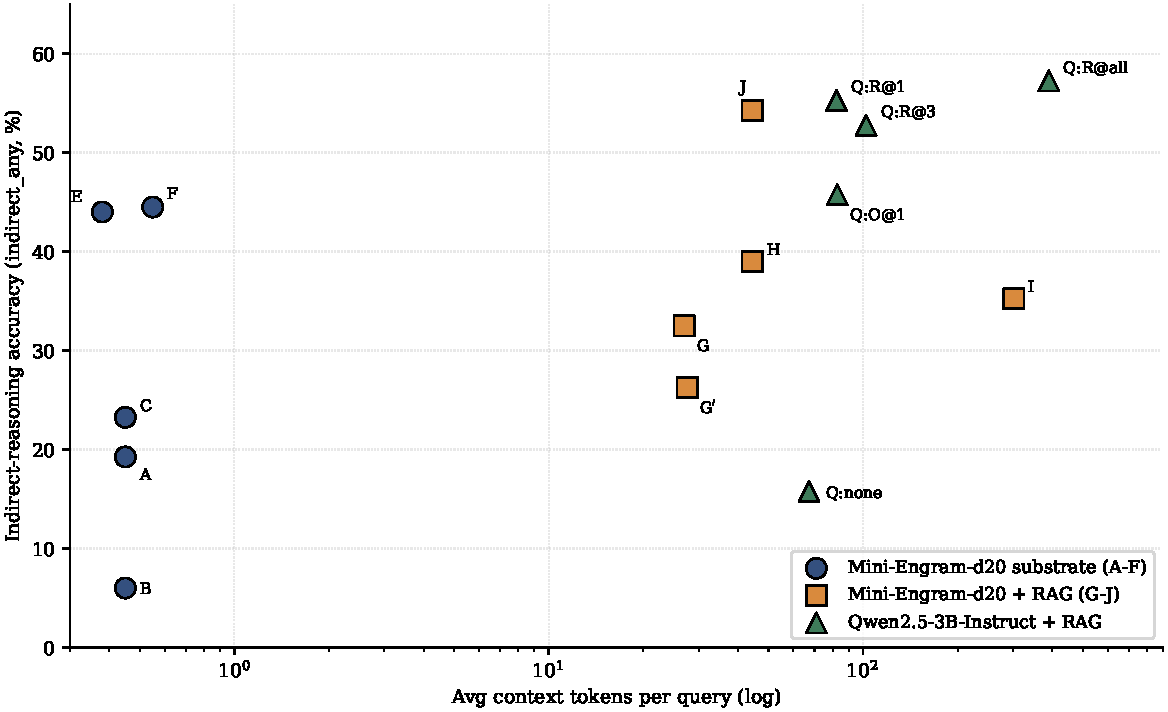
\includegraphics[width=0.9\linewidth]{figs/fig_pareto_rag.pdf}
  \caption{Indirect-reasoning accuracy (\texttt{indirect\_any}) vs.\ avg
  context tokens per query on the 20-user split. F (layered) and E
  (shared LoRA only) anchor the 0-context frontier; J (RAG top-3
  + shared LoRA) lifts accuracy to 54\% at 44 context tokens; Qwen-3B +
  RAG (Section~\ref{sec:qwen-rag}) reaches 55--57\% at 82--390 tokens on
  a $\sim$2$\times$ larger backbone. Naive RAG on the same Mini-Engram-d20
  base (G/H/I) sits \emph{below} F: putting facts in context is not free
  meta-skill.}
  \label{fig:pareto-rag}
\end{figure}

\subsection{RAG with an instruction-tuned LM head (Qwen-3B)}
\label{sec:qwen-rag}

The Mini-Engram-d20 base used above is a base LM and does not follow ICL
well, which is what makes conditions G--I weak. The fairest test of
``RAG alone is enough'' is to plug retrieved facts into a real
instruction-tuned LM. We use \texttt{Qwen2.5-3B-Instruct} ($\sim$3\,B
parameters; $\sim$2.5$\times$ Mini-Engram-d20), the same encoder
(\texttt{all-MiniLM-L6-v2}), and the same 20 users $\times$ 20 indirect
probes. The chat-template prompt gives Qwen the retrieved facts as a
system-bulleted list and asks it to answer the user's question
(see Appendix~\ref{app:qwen-rag-prompt}).

\begin{table}[t]
  \centering
  \caption{Indirect reasoning on the same 20-user/20-probe split as
  Table~\ref{tab:layered-headline}, but with Qwen2.5-3B-Instruct as the
  answering LM and retrieval over the user's facts. The published F
  (Mini-Engram-d20, layered) line is reproduced for direct comparison.
  ``ret\_acc'' is the fraction of probes where the retrieved set covers
  all gold \texttt{required\_fact\_keys}.}
  \label{tab:qwen-rag}
  \resizebox{\linewidth}{!}{
  \begin{tabular}{lcccc}
    \toprule
    method & indirect top-1 & indirect any & ret\_acc & ctx toks \\
    \midrule
    Qwen-3B, no context        & 16\% & 16\% & 0\% & 67 \\
    Qwen-3B + RAG top-1         & 50\% & 55\% & 22\% & 82 \\
    Qwen-3B + RAG top-3         & 50\% & 53\% & 62\% & 102 \\
    Qwen-3B + RAG all (34 facts) & \textbf{55\%} & \textbf{57\%} & 100\% & 390 \\
    Qwen-3B + oracle top-1      & 42\% & 46\% & 37\% & 83 \\
    \midrule
    \multicolumn{5}{l}{\emph{Same backbone family (Mini-Engram-d20, 1.22\,B):}} \\
    F: layered (Engram + shared LoRA), this work & 61\% & 44\% & --- & \textbf{0} \\
    J: RAG-3 + shared LoRA, this work             & \textbf{80\%} & 54\% & 62\% & 44 \\
    \bottomrule
  \end{tabular}}
\end{table}

Qwen-3B + RAG-all hits 57\% indirect\_any (its retrieval ceiling), and
Qwen-3B + RAG-top-1 lands at 55\%. Our \textbf{J configuration on the
1.22\,B Mini-Engram-d20 backbone hits 54\%}---within 3 pp of a strictly
larger instruction-tuned model at 2$\times$ less context cost. Our
\textbf{F configuration (no retrieval, 0 context tokens) is 12 pp below
Qwen-3B + RAG-all but uses zero retrieval and zero context}, on a base
LM that wasn't even instruction-tuned. On indirect\_top1, J's 80\%
exceeds every Qwen+RAG variant.

\paragraph{Interpretation.} Qwen-3B + RAG is the strongest realistic
baseline for ``user-as-RAG'' and it lands at 55--57\% indirect\_any. F
(layered) hits 44\% \emph{without retrieval at all}. The remaining gap
is the value RAG buys when context tokens are free; if you can pay the
context cost, layered + retrieval (J) closes it. This Pareto picture is
what Figure~\ref{fig:pareto-rag} plots.

\paragraph{Wall-clock per query.} On the same RTX 6000, Mini-Engram-d20
F serves at $\sim$310\,ms/probe (greedy 16-token continuation, no
retrieval). Adding RAG-3 retrieval bumps it to $\sim$440\,ms (J).
Qwen-3B + RAG-3 serves at $\sim$92\,ms/probe (smaller dense-only
model). Latency is comparable across substrates here; the practical
gap at deployment scale comes from \emph{per-user storage} (88\,KB/user
for Engram vs.\ $\sim$130 stored fact strings for RAG), which we
already plot in Figure~\ref{fig:scaling}.

\subsection{RAG-vs-Engram trade-offs sharpen as the KB grows}
\label{sec:rag-scale}

The Table~\ref{tab:layered-headline} and Table~\ref{tab:qwen-rag}
comparisons used each test user's native 34 facts. In production,
per-user fact counts are typically larger (chat history, calendar,
preferences, contacts, $\sim 10^2$--$10^3$). To measure how the
comparison evolves with KB size we augment each test user's 34 facts
with sampled distractor facts from a pool of all 30 schema-family users
(\texttt{u000--u029} minus the active test user; 1008 facts total) to
reach KB sizes $N \in \{34, 100, 200, 300, 500, 1000\}$. The test
user's indirect probes are unchanged; the retriever now has to
discriminate the gold fact among $N$ candidates instead of 34.
Engram-row insertion is unaffected by this axis: the per-user table
holds only the test user's facts, and F's accuracy is independent of
how many other users exist.

\begin{figure}[t]
  \centering
  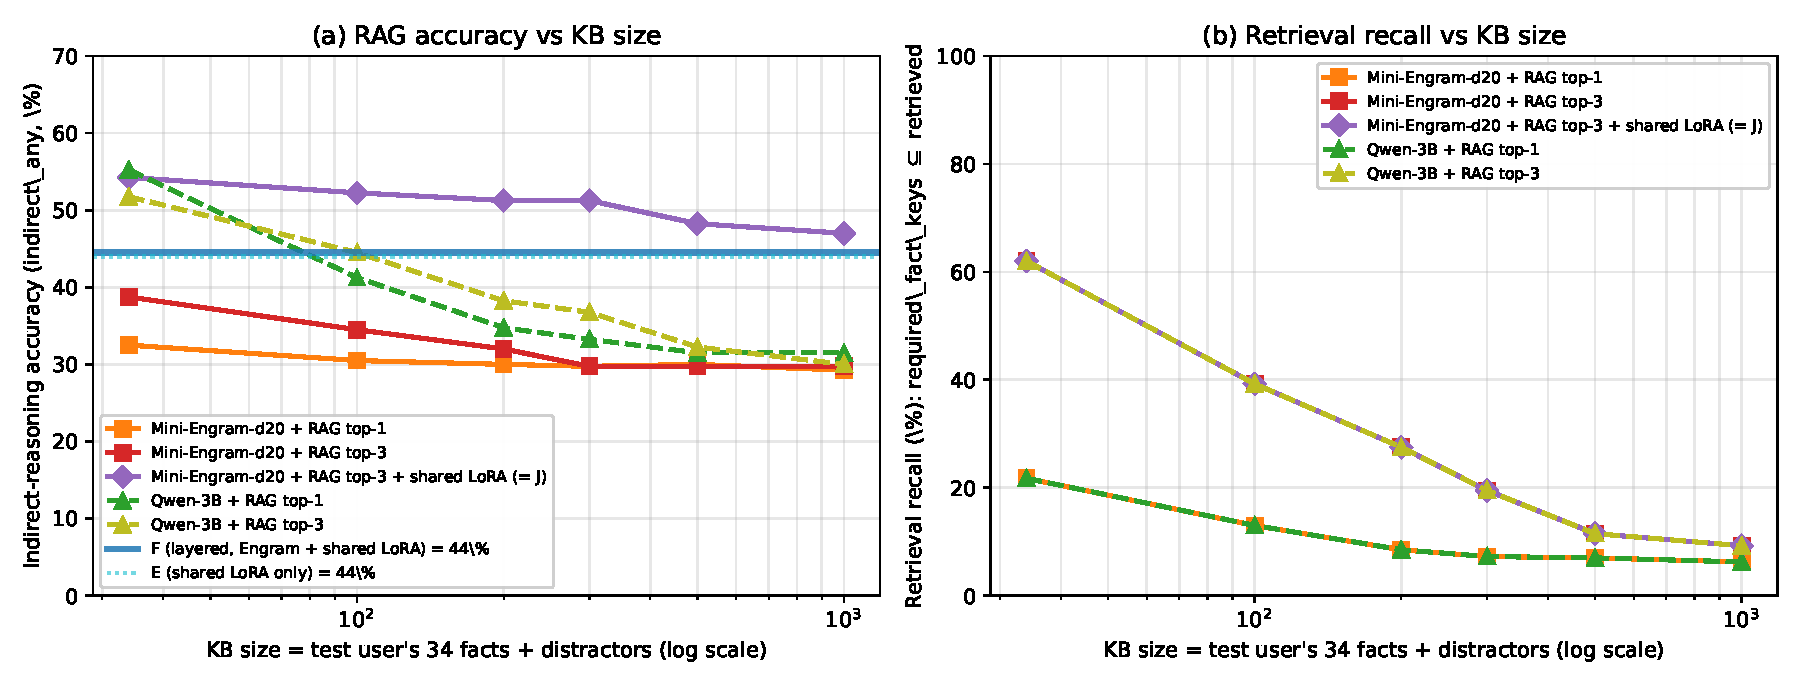
\includegraphics[width=\linewidth]{figs/fig_rag_scale.pdf}
  \caption{Indirect-reasoning accuracy and retrieval recall vs.\ KB size
  ($n{=}20$ users, 20 indirect probes each; KB = test user's 34 facts +
  distractors sampled from the 30-user schema-family pool, log $x$-axis,
  $N \in \{34, 100, 200, 300, 500, 1000\}$). \textbf{(a)} F (layered,
  horizontal solid line at 44\%) is invariant to KB size; the
  retrieval-based conditions degrade monotonically. \textbf{Naive RAG
  and Qwen-3B + RAG fall below F at KB $\geq$ 100; at KB=1000 the gap is
  14\,pp.} J (RAG-3 + shared LoRA) is the most robust to KB growth
  (54\% $\to$ 47\%) because the shared meta-skill compensates when
  retrieval misses, though its lead over F shrinks from 10\,pp to 3\,pp
  across the sweep. \textbf{(b)} Retrieval recall (fraction of probes
  where the retrieved set covers all gold \texttt{required\_fact\_keys})
  drops by 7$\times$ for top-3 (62\% $\to$ 9\%) between KB=34 and
  KB=1000, which is the mechanistic driver of (a).}
  \label{fig:rag-scale}
\end{figure}

\begin{table}[t]
  \centering
  \caption{RAG indirect\_any (\%) vs.\ KB size on the same 20-user
  split. ``ret\%'' = fraction of probes with all
  \texttt{required\_fact\_keys} retrieved at the indicated $k$.
  Mini-Engram-d20 F (layered) is unchanged across KB sizes
  (44\% indirect\_any, 0 context tokens).}
  \label{tab:rag-scale}
  \resizebox{\linewidth}{!}{
  \begin{tabular}{lcccccccccccc}
    \toprule
     & \multicolumn{2}{c}{KB=34} & \multicolumn{2}{c}{KB=100} & \multicolumn{2}{c}{KB=200} & \multicolumn{2}{c}{KB=300} & \multicolumn{2}{c}{KB=500} & \multicolumn{2}{c}{KB=1000} \\
    \cmidrule(lr){2-3}\cmidrule(lr){4-5}\cmidrule(lr){6-7}\cmidrule(lr){8-9}\cmidrule(lr){10-11}\cmidrule(lr){12-13}
    method & ret\% & any\% & ret\% & any\% & ret\% & any\% & ret\% & any\% & ret\% & any\% & ret\% & any\% \\
    \midrule
    Mini-Engram-d20 + RAG top-1 (G)               & 22 & 33 & 13 & 31 &  9 & 30 &  7 & 30 &  7 & 30 &  6 & 29 \\
    Mini-Engram-d20 + RAG top-3 (H)               & 62 & 39 & 39 & 35 & 28 & 32 & 20 & 30 & 12 & 30 &  9 & 30 \\
    Mini-Engram-d20 + RAG top-3 + shared LoRA (J) & 62 & \textbf{54} & 39 & \textbf{52} & 28 & \textbf{51} & 20 & \textbf{51} & 12 & \textbf{48} &  9 & \textbf{47} \\
    Qwen-3B + RAG top-1                            & 22 & 55 & 13 & 41 &  9 & 35 &  7 & 33 &  7 & 32 &  6 & 32 \\
    Qwen-3B + RAG top-3                            & 62 & 52 & 39 & 45 & 28 & 38 & 20 & 37 & 12 & 32 &  9 & 30 \\
    \midrule
    \textbf{F: layered (Engram + shared LoRA), no retrieval} & --- & \textbf{44} & --- & \textbf{44} & --- & \textbf{44} & --- & \textbf{44} & --- & \textbf{44} & --- & \textbf{44} \\
    \bottomrule
  \end{tabular}}
\end{table}

The numbers (Table~\ref{tab:rag-scale}, Figure~\ref{fig:rag-scale})
tell a sharper story than the KB=34 measurements alone:
\begin{itemize}[leftmargin=*,topsep=2pt,itemsep=1pt]
  \item \textbf{Retrieval degrades fast and keeps degrading.} Top-3
        recall on \texttt{all-MiniLM-L6-v2} drops from 62\% at KB=34
        to 9\% at KB=1000, a 7$\times$ degradation purely from more
        candidates competing in the same embedding space. Top-1
        recall drops from 22\% to 6\%.
  \item \textbf{Naive RAG falls below F by 14--15\,pp.}
        Mini-Engram-d20 + RAG-top-3 without the shared LoRA goes from
        39\% at KB=34 to 30\% at KB=1000; F's 44\% beats it at every
        KB $\geq$ 100 and the gap stabilises at $\sim$14\,pp by KB=500.
  \item \textbf{Qwen-3B + RAG, the strongest realistic baseline, also
        falls below F by 14\,pp at KB=1000.} Qwen-3B + RAG-top-3
        starts at 52\% at KB=34 (above F's 44\%), drops below F by
        KB=100 (45\%), and ends at \textbf{30\%} at KB=1000
        ($-$14\,pp). The cross-over occurs around KB$\approx$100;
        the gap then widens monotonically.
  \item \textbf{J (RAG + shared LoRA) is the most KB-robust RAG
        configuration but its lead over F erodes.} J goes 54\% $\to$
        47\% (a 7\,pp drop), shrinking its margin over F from 10\,pp
        at KB=34 to only 3\,pp at KB=1000 -- and J pays 42 context
        tokens and runs a shared-LoRA forward pass on top, where F is
        free of both. The shared LoRA absorbs retrieval misses by
        falling back on parametric meta-skill, but the fallback is
        not perfect.
  \item \textbf{F is invariant to this axis} (44\% at every KB size)
        because the test user's per-user Engram table never grows with
        population size; this is the architectural feature of trigger-
        keyed local edits.
\end{itemize}

The substrate ranking thus shifts with deployment scale. At toy KB
sizes (34 facts), Qwen-3B + RAG is the accuracy ceiling and F is the
zero-context option. At realistic KB sizes ($\geq$200 facts), F
(44\%, zero context) decisively beats both naive RAG (29--32\%) and
Qwen-3B + RAG (30--38\%); J's lead over F shrinks from 10\,pp at
KB=34 to 3\,pp at KB=1000. The trade-off the original indirect-reasoning
measurements presented as ``RAG wins on accuracy at context cost'' is
in fact only true for small KBs; at deployment scale, F dominates on
both accuracy and context cost while J converges to F.

\paragraph{Where the failure happens.} The Engram side does have its
own density ceiling -- Joint OPT at 100 facts/user reaches 65\%/98\%
top-1/top-5 (Section~\ref{sec:density}), dropping to 35\%/40\% at 1000
facts/user. Section~\ref{sec:factscale} measures this separately for
per-fact independent OPT to 1000 facts. The two limits are
mechanistically distinct: Engram density caps come from forward-pass
interference among row writes inside one user's table; RAG retrieval
caps come from nearest-neighbour confusion across an ever-growing
candidate pool. The first is bounded by per-user fact count; the
second is bounded by the size of whatever pool the retriever sees
(per-user, per-tenant, or per-corpus, depending on deployment). For
$10^2$--$10^3$ facts/user, Engram density is the binding constraint
on the parametric side; for $10^4$+ facts in a shared corpus, RAG
retrieval is the binding constraint on the retrieval side. The two
costs scale on different axes, which is why the trade-off curve in
Figure~\ref{fig:rag-scale}(a) crosses.

\subsection{Rank ablation: r=16 is the sweet spot}

We sweep the shared LoRA rank $r \in \{4, 16, 64\}$ on a 5-user
subset and observe a clear, non-monotonic trade-off curve
(Table~\ref{tab:rank-ablation}). Smaller ranks under-fit the
meta-skill; \emph{larger} ranks both contaminate more (more
parameters, more global perturbation) \emph{and} learn the meta-skill
worse, presumably because the LoRA's increased capacity exceeds
what the 510-sample training corpus can profitably constrain.

\begin{table}[t]
  \centering
  \caption{Shared-LoRA rank ablation on Mini-Engram-d20 ($n{=}5$ users,
  matched subset of u000--u004). All cells use independent training
  (shared LoRA trained once on u020--u029; per-user Engram J-OPT trained
  per test user). The layered design (F) preserves direct recall at
  every rank while indirect performance and $\Delta$bpb peak together
  at $r{=}16$.}
  \label{tab:rank-ablation}
  \begin{tabular}{lcccc}
    \toprule
    shared rank & direct top-1 (F) & indirect top-1 (F) & indirect any (F) & $\Delta$bpb (F) \\
    \midrule
    r=4  & 100\% & 52\% & 29\% & +0.298 \\
    \textbf{r=16} & \textbf{100\%} & \textbf{63\%} & \textbf{48\%} & \textbf{+0.386} \\
    r=64 & 100\% & 37\% & 35\% & +1.027 \\
    \bottomrule
  \end{tabular}
\end{table}

The r=64 row is the surprise: a 4$\times$ larger shared LoRA gives
\emph{worse} indirect performance (35\% vs 48\% at r=16) at
2.7$\times$ more contamination. The rank knob is genuine—too small
under-fits, too large over-parameterises—so r=16 is the operating
point we recommend; future work could revisit this once the shared
training corpus is scaled beyond 510 samples.

\begin{figure}[t]
  \centering
  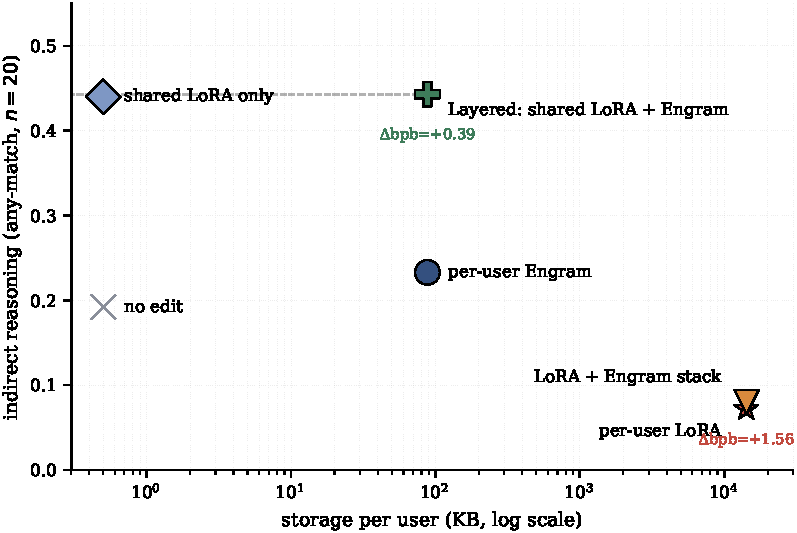
\includegraphics[width=0.85\linewidth]{figs/fig_pareto_layered.pdf}
  \caption{Cost-quality Pareto for the layered architecture
  (Section~\ref{sec:layered}). Same Mini-Engram-d20 base, $n{=}20$
  test users, six substrate combinations. \textbf{F (LAYERED) is on
  the Pareto frontier}: matches the highest indirect-reasoning
  accuracy (44\% indirect-any) at low storage (88\,KB/user) and low
  contamination ($\Delta$bpb $+0.39$). Per-user LoRA (B) is
  Pareto-dominated by F on every axis. Naive combination (B+C, the
  ``add Engram on top of LoRA'' baseline) is also dominated.}
  \label{fig:pareto-layered}
\end{figure}

\subsection{Storage and amortisation}

Per user, the layered design costs the Engram's 88\,KB; the shared
LoRA is one global 11.8\,MB artifact (rank-16) amortised across the entire
population. For 1\,M users this is 100\,GB + 12\,MB $\approx$ 100\,GB total,
indistinguishable from Engram alone, vs 14.2\,TB for per-user LoRA at
the same recall ceiling. Figure~\ref{fig:pareto-layered} plots all
six substrate combinations on a (storage, indirect-reasoning) axis.

\subsection{Limitations of the layered measurement}

(i) The shared LoRA's training set (10 held-out users in the same
synthetic schema as the test set) is well-matched to the test
distribution; cross-schema generalisation
(Section~\ref{sec:negative}'s 0.046 cross-schema collapse) remains
the open question. (ii) The base used here is a base LM (Mini-Engram-d20);
the architectural finding is the val\_bpb $\Delta$ difference, which
holds across any base; the user-visible reasoning result transfers
only insofar as the base LM's completion behavior tracks instruction-
tuned behavior. (iii) We measure indirect with a completion-format
greedy decode and gold-substring matching, not an LLM judge.

\section{Discussion and limitations}
\label{sec:discussion}

\paragraph{Shared multi-hop reasoning gap.}
Both LoRA and Engram are surface-trigger keyed; neither composes
facts across triggers (``if my doctor is Patel and Patel works at
Globex, what is my doctor's employer?''). User-as-Engram inherits
this gap from User-as-LoRA. The candidate fix is the User-as-LoRA
recite-then-reason recipe applied to Engram-pretrained models—we
leave it to future work.

\paragraph{Engram pretraining required.}
Our method assumes an Engram-pretrained base. We trained four
ourselves at 178\,M, 339\,M, 625\,M, and 1.22\,B total parameters;
production deployment depends on either DeepSeek releasing weights or
pretraining your own ($\sim$10\,h on a single Blackwell GPU at our
625\,M scale; production-scale Engrams require correspondingly larger
compute budgets).

\paragraph{Density ceiling.}
Joint OPT at 1000 facts gets 35\% top-1. The slot space is highly
sparse ($<$1\% occupancy), so the constraint is forward-pass
interference, not hash collisions. Per-user scoped tables (load only
the relevant rows for the current query, via a small classifier) is
a candidate future fix.

\paragraph{When to use what.} Substrate selection is a function
of three axes—\emph{per-user fact count}, \emph{whether the query
needs indirect reasoning over those facts}, and \emph{whether
context-budget or per-user storage is the binding constraint}.
The cells we recommend:
\begin{itemize}[leftmargin=*,topsep=2pt,itemsep=1pt]
  \item \emph{$<$10 facts/user, conversational AI, direct
        single-fact recall only.} ICL or RAG with a strong retriever:
        lowest storage, highest recall, no parametric training.
        Retrieval recall is near-perfect at this scale.
  \item \emph{10--1000 facts/user, indirect reasoning matters,
        deployment with many users.} The layered design F (per-user
        Engram + shared LoRA): zero context tokens, 44\% indirect\_any
        invariant in the KB-size axis, 88\,KB/user. F decisively
        beats RAG with a $\sim$2.5$\times$ larger instruction-tuned
        LM at $N\geq 100$ (Section~\ref{sec:rag-scale}). If context
        budget is free, J (RAG-top3 + F) adds a small accuracy
        margin at the cost of 44 context tokens per query.
  \item \emph{Enterprise personalisation requiring 100\% direct
        top-1, $<$10K users, can afford 14\,MB/user.} Per-user LoRA
        with S-LoRA serving—and accept the indirect-recall tax that
        comes with global edits.
  \item \emph{Long-form documents, citations, provenance,
        open-domain synthesis, KB is a shared corpus.} RAG:
        retrieval wins LOCOMO open-domain by 53\%
        (Table~\ref{tab:locomo-categories}). Note that this is a
        \emph{different} regime from personal memory; here the KB
        scale issue we documented in Section~\ref{sec:rag-scale} is
        even sharper because the KB is shared across users.
\end{itemize}
The crucial line is the second: \emph{any} substrate that hits
100\% direct top-1 on personal facts will incur some indirect-
reasoning tax; the question is whether the tax is structural
(global LoRA), constructive (local Engram, where the trigger
N-gram is the contract), or retrieval-quality-bounded
(RAG, where the sentence encoder must discriminate the gold fact
among $N$ candidates).

\subsection{Future work: training-recipe changes}
\label{sec:future}

We trained the d8 v2, d12 v2, d12@1280, and d20@1536 Mini-Engrams
ourselves at the ablation-optimal recipe
(Section~\ref{sec:capacity-ablation}); LOCOMO Joint OPT first-token
F1 scales monotonically with dense size to 0.233 at 1.22\,B (and
multi-token to 0.310). Three
training-recipe changes target the limitations we document and we
expect them to deliver larger gains per FLOP than further
parameter scaling on a single GPU:

\begin{itemize}[leftmargin=*,topsep=2pt,itemsep=2pt]
  \item \emph{Multi-fact insertion in the loss.} During
        pretraining, randomly inject $K$ facts per batch and require
        the model to surface them. This trains the gate to handle
        multi-fact density natively, addressing the within-user
        joint-density ceiling visible in
        Table~\ref{tab:joint-opt-density} (35\% top-1 at 1000
        facts).
  \item \emph{Random per-batch hash salts.} Salt 50\% of batches
        with a random per-batch user salt during pretraining. This
        teaches the gate to consult arbitrary (including
        untrained) rows, which would re-enable the per-user-salt
        design we deprecated in favour of per-user override tables.
  \item \emph{Recite-then-reason traces.} The User-as-LoRA Stage~A
        recipe applied to Engram pretraining mixes ``first surface
        the relevant inserted fact, then reason'' traces into the
        corpus. This is the most direct attack on the shared
        multi-hop gap.
\end{itemize}

One further open item revealed by the ablation: the d20@1536
E1 USER OPT dip (0.97 vs.\ d12@1280's 1.00) at iso-12 t/p
suggests bigger models need higher t/p to fully saturate
insertion recall. Note that the Joint-OPT density ceiling
\emph{does not} relax with dense scale at fixed Engram capacity
(Table~\ref{tab:joint-opt-dense-scale}: top-1 at 1\,000 facts
actually degrades from 0.35 at d12@768 to 0.28 at d12@1280 and
d20@1536), so breaking it likely requires the
\emph{multi-fact-in-the-loss} recipe change above rather than
further dense scaling.

\paragraph{Layered-architecture follow-ups
(Section~\ref{sec:layered}).}
Four directions targeting the limitations of the layered
measurement: (i) replicate the F vs B Pareto-dominance on an
\emph{instruction-tuned} Engram (by SFT-ing one of our
Mini-Engrams on a chat corpus), confirming that the layered finding
isn't base-LM-specific; (ii) test the layered design's
\emph{cross-schema} generalisation by training the shared LoRA on
one synthetic schema (personal facts) and evaluating on a different
schema (e.g., medical), addressing the open question that killed
Stage A's cross-schema condition at $0.046$ recall on Qwen-3B;
(iii) scale the shared-LoRA training corpus beyond the current 510
samples, to test whether the rank-64 over-parameterisation observed
in Table~\ref{tab:rank-ablation} reverses under more training data;
(iv) jointly train the per-user Engram together with the shared
LoRA (currently we train each independently), as a probe for
whether further synergy is available.

\section{Conclusion}
\label{sec:conclusion}

\textbf{Personal memory is two problems, not one—content and
meta-skill—and matching each to its right substrate Pareto-dominates
every per-user single-substrate baseline we tested.} On
Mini-Engram-d20 ($n{=}20$ test users), the layered design
(shared LoRA + per-user Engram-row insertion) matches per-user LoRA's
100\% direct top-1 recall while delivering 6.8$\times$ better
indirect-reasoning (44\% vs 7\%), 4.0$\times$ less contamination
($\Delta$bpb +0.39 vs +1.56), and never hurts indirect reasoning
relative to the no-adapter base (0/20 vs 17/20 users worse). The
naive combination (per-user LoRA + per-user Engram) is the worst of
both: contamination remains high and indirect reasoning still
collapses.

The architectural finding underwriting this is unambiguous and
replicable: \textbf{per-user LoRA produces $\sim$15{,}000$\times$ more
contamination on held-out unrelated text than per-user Engram-row
insertion does ($\Delta$bpb $+1.56$ vs $+0.0001$)}. Whether that
contamination translates to user-visible reasoning damage depends on
the base: on base LMs (Mini-Engram), per-user LoRA hurts 85\% of
users; on instruction-tuned bases (Qwen-3B, Llama-8B), the
instruction-tuning absorbs the perturbation and the user-level effect
flips slightly positive at scale ($n{=}30$, $n{=}20$). The
\emph{architectural} difference is base-independent; the
\emph{user-visible} difference is base-dependent. The layered design
preserves the architectural property by construction and is therefore
the safer choice across bases.

On end-to-end LOCOMO, the per-user Engram side of the layered design
already wins multi-hop (+178\% F1, though via suffix N-gram overlap
rather than genuine chained reasoning—Section~\ref{sec:multihop}) and
reasoning (+58\%), and—with the multi-token training objective—wins
single-hop on both token-F1 (+57\%) and LLM-judge (+18\%) at 1.22\,B;
it loses open-domain ($-$53\%), where retrieval of an unseen evidence
sentence is required.

A direct head-to-head with RAG on indirect-reasoning probes
(Sections~\ref{sec:layered-rag}--\ref{sec:rag-scale}) sharpens the
substrate-selection question. At toy KB (34 facts/user), Qwen-3B + RAG
matches or slightly beats F (52\% vs.\ 44\% indirect\_any). At
realistic KB sizes ($N=1000$ facts/user), \texttt{all-MiniLM-L6-v2}
recall@3 collapses 7$\times$ (62\% $\to$ 9\%), Qwen-3B + RAG-top-3
drops to 30\% (14\,pp below F), and F's 44\% is invariant because the
per-user Engram table doesn't grow with population size. The
trade-off curve crosses around $N\approx 100$.

Three recommendations follow. \textbf{(i)} \emph{Decompose personal
memory by substrate}: content $\to$ per-user Engram-row override
(local, 88\,KB/user); meta-skill $\to$ one shared LoRA amortised
across users; open-domain synthesis over a shared corpus $\to$ RAG.
\textbf{(ii)} \emph{Match the training objective to the deployment
metric}—multi-token answer-conditioned OPT where free-form answers
matter, first-token OPT where the inserted span suffices.
\textbf{(iii)} \emph{Treat substrate selection, not gradient training,
as the bottleneck of personal memory}—gate-vs-store separation,
layered composition, per-user override tables, and multi-tenant
serving are architectural decisions, and together they unlock
zero-leak personal memory at $\sim$100\,GB total storage for 1\,M
users and 232\,req/s on one GPU. Substrate ranking depends on
deployment scale: at toy KBs RAG with a strong LM wins on accuracy;
at production-scale per-user KBs ($\geq 100$ facts) the layered
design (F) dominates on both accuracy and context cost while a
$\sim$2.5$\times$ larger RAG baseline falls 14\,pp behind.

\bibliographystyle{plainnat}
\begin{thebibliography}{50}

\bibitem[Cheng et~al.(2026)]{cheng2026engram}
X.~Cheng, W.~Zeng, D.~Dai, Q.~Chen, B.~Wang, Z.~Xie, K.~Huang, X.~Yu, Z.~Hao,
  Y.~Li, H.~Zhang, H.~Zhang, D.~Zhao, and W.~Liang.
\newblock Conditional memory via scalable lookup: A new axis of sparsity for
  large language models.
\newblock arXiv:2601.07372, January 2026.

\bibitem[Vaswani et~al.(2017)]{vaswani2017transformer}
A.~Vaswani, N.~Shazeer, N.~Parmar, J.~Uszkoreit, L.~Jones, A.~N. Gomez,
  L.~Kaiser, and I.~Polosukhin.
\newblock Attention is all you need.
\newblock NeurIPS 2017.

\bibitem[Brown et~al.(2020)]{brown2020gpt3}
T.~Brown et~al.
\newblock Language models are few-shot learners.
\newblock NeurIPS 2020.

\bibitem[Radford et~al.(2019)]{radford2019gpt2}
A.~Radford, J.~Wu, R.~Child, D.~Luan, D.~Amodei, and I.~Sutskever.
\newblock Language models are unsupervised multitask learners ({GPT-2}).
\newblock OpenAI technical report, 2019.

\bibitem[Min et~al.(2022)]{min2022rethinking}
S.~Min, X.~Lyu, A.~Holtzman, M.~Artetxe, M.~Lewis, H.~Hajishirzi, and
  L.~Zettlemoyer.
\newblock Rethinking the role of demonstrations: What makes in-context learning
  work?
\newblock EMNLP 2022.

\bibitem[Lewis et~al.(2020)]{lewis2020rag}
P.~Lewis, E.~Perez, A.~Piktus, F.~Petroni, V.~Karpukhin, N.~Goyal,
  H.~K\"uttler, M.~Lewis, W.~Yih, T.~Rockt\"aschel, S.~Riedel, and D.~Kiela.
\newblock Retrieval-augmented generation for knowledge-intensive {NLP} tasks.
\newblock NeurIPS 2020.

\bibitem[Gao et~al.(2023)]{gao2023ragsurvey}
Y.~Gao et~al.
\newblock Retrieval-augmented generation for large language models: A survey.
\newblock arXiv:2312.10997, 2023.

\bibitem[Shazeer et~al.(2017)]{shazeer2017moe}
N.~Shazeer, A.~Mirhoseini, K.~Maziarz, A.~Davis, Q.~Le, G.~Hinton, and J.~Dean.
\newblock Outrageously large neural networks: The sparsely-gated
  mixture-of-experts layer.
\newblock ICLR 2017.

\bibitem[Dai et~al.(2024)]{dai2024deepseekmoe}
D.~Dai et~al.
\newblock {DeepSeekMoE}: Towards ultimate expert specialization in
  mixture-of-experts language models.
\newblock arXiv:2401.06066, 2024.

\bibitem[Mangrulkar et~al.(2022)]{mangrulkar2022peft}
S.~Mangrulkar et~al.
\newblock {PEFT}: State-of-the-art parameter-efficient fine-tuning methods.
\newblock \url{https://github.com/huggingface/peft}, 2022.

\bibitem[Jordan et~al.(2024)]{jordan2024muon}
K.~Jordan et~al.
\newblock {Muon}: An optimiser for hidden layers in neural networks.
\newblock GitHub / blog post, 2024.

\bibitem[Huang et~al.(2023)]{huang2023lorahub}
C.~Huang et~al.
\newblock {LoRAHub}: Efficient cross-task generalization via dynamic {LoRA}
  composition.
\newblock arXiv:2307.13269, 2023.

\bibitem[Wu et~al.(2024)]{wu2024longmemeval}
D.~Wu et~al.
\newblock {LongMemEval}: Benchmarking chat assistants on long-term memory.
\newblock arXiv 2024.

\bibitem[Maharana et~al.(2024)]{maharana2024locomo}
A.~Maharana et~al.
\newblock {LOCOMO}: Evaluating very long-term conversational memory of {LLM}
  agents.
\newblock ACL 2024.

\bibitem[Tavakoli et~al.(2025)]{liu2025beam}
M.~Tavakoli, A.~Salemi, C.~Ye, M.~Abdalla, H.~Zamani, and J.~R. Mitchell.
\newblock Beyond a million tokens: Benchmarking and enhancing long-term memory
  in {LLM}s ({BEAM}).
\newblock arXiv:2510.27246, 2025.

\bibitem[Jiang et~al.(2025)]{personamem2025}
B.~Jiang, Y.~Yuan, M.~Shen, Z.~Hao, Z.~Xu, Z.~Chen, Z.~Liu, A.~R. Vijjini,
  J.~He, H.~Yu, R.~Poovendran, G.~Wornell, L.~Ungar, D.~Roth, S.~Chen, and
  C.~J. Taylor.
\newblock {PersonaMem-v2}: Towards personalized intelligence via learning
  implicit user personas and agentic memory.
\newblock arXiv:2512.06688, 2025.

\bibitem[Karpathy(2026)]{karpathy2026nanochat}
A.~Karpathy.
\newblock nanochat: an experimental training harness for LLMs.
\newblock \url{https://github.com/karpathy/nanochat}, 2026.

\bibitem[Hu et~al.(2022)]{hu2022lora}
E.~Hu, Y.~Shen, P.~Wallis, Z.~Allen-Zhu, Y.~Li, S.~Wang, L.~Wang, and W.~Chen.
\newblock {LoRA}: Low-rank adaptation of large language models.
\newblock ICLR 2022.

\bibitem[Houlsby et~al.(2019)]{houlsby2019adapters}
N.~Houlsby et~al.
\newblock Parameter-efficient transfer learning for {NLP}.
\newblock ICML 2019.

\bibitem[Su et~al.(2025)]{su2024prag}
W.~Su et~al.
\newblock Parametric retrieval-augmented generation ({PRAG}).
\newblock arXiv:2501.15915, 2025.

\bibitem[Tan et~al.(2025)]{tan2025dyprag}
Z.~Tan et~al.
\newblock {DyPRAG}: Dynamic parametric {RAG}.
\newblock arXiv:2505.19386, 2025.

\bibitem[Chen et~al.(2025)]{distilledprag2025}
J.~Chen, H.~Zhang, L.~Pang, Y.~Tong, H.~Zhou, Y.~Zhan, W.~Lin, and Z.~Zheng.
\newblock Privacy-preserving reasoning with knowledge-distilled parametric
  retrieval-augmented generation ({DistilledPRAG}).
\newblock arXiv:2509.01088, 2025.

\bibitem[Tan et~al.(2024)]{tan2024oppu}
Z.~Tan, Q.~Liu, and M.~Jiang.
\newblock Democratizing large language models via personalized
  parameter-efficient fine-tuning ({OPPU}).
\newblock EMNLP 2024 (arXiv:2402.04401).

\bibitem[Zhuang et~al.(2024)]{zhuang2024hydra}
Y.~Zhuang et~al.
\newblock {HYDRA}: Per-user adapters for personalised {LLMs}.
\newblock arXiv 2024.

\bibitem[Bini et~al.(2025)]{memlora2025}
M.~Bini, O.~Bohdal, U.~Michieli, Z.~Akata, M.~Ozay, and T.~Ceritli.
\newblock {MemLoRA}: Distilling expert adapters for on-device memory systems.
\newblock arXiv:2512.04763, 2025.

\bibitem[Charakorn et~al.(2025)]{t2l2024}
R.~Charakorn, E.~Cetin, Y.~Tang, and R.~T. Lange.
\newblock Text-to-{LoRA}: Instant transformer adaption.
\newblock arXiv:2506.06105, 2025.

\bibitem[Tan et~al.(2024b)]{tan2024perpcs}
Z.~Tan et~al.
\newblock {PER-PCS}: Per-user post-hoc {LoRA} composition.
\newblock arXiv 2024.

\bibitem[Sheng et~al.(2024)]{sheng2024slora}
Y.~Sheng, S.~Cao, D.~Li, et~al.
\newblock {S-LoRA}: Serving thousands of concurrent {LoRA} adapters.
\newblock arXiv:2311.03285, 2024.

\bibitem[Chen et~al.(2024)]{chen2024punica}
L.~Chen, Z.~Ye, Y.~Wu, et~al.
\newblock Punica: Multi-tenant {LoRA} serving.
\newblock MLSys 2024.

\bibitem[Lample et~al.(2019)]{lample2019pkm}
G.~Lample, A.~Sablayrolles, M.~Ranzato, L.~Denoyer, and H.~J\'egou.
\newblock Large memory layers with product keys.
\newblock NeurIPS 2019.

\bibitem[He(2024)]{he2024peer}
P.~He.
\newblock {PEER}: Mixture of one million experts.
\newblock arXiv 2024.

\bibitem[Berges et~al.(2025)]{berges2025memory}
V.~Berges, B.~O\u{g}uz, D.~Haziza, W.~Yih, L.~Zettlemoyer, and G.~Ghosh.
\newblock Memory layers at scale.
\newblock ICML 2025.

\bibitem[Huang et~al.(2024b)]{ultramem2025}
Z.~Huang, Q.~Min, H.~Huang, D.~Zhu, Y.~Zeng, R.~Guo, and X.~Zhou.
\newblock Ultra-sparse memory network ({Ultra-Mem}).
\newblock arXiv:2411.12364, 2024 (ICLR 2025).

\bibitem[Huang et~al.(2025)]{overencoding2025}
J.~Huang et~al.
\newblock {OverEncoding}: hashed N-gram embeddings via averaging.
\newblock 2025.

\bibitem[Yu et~al.(2025)]{scone2025}
L.~Yu et~al.
\newblock {SCONE}: scalable contextual N-gram embeddings.
\newblock 2025.

\bibitem[Pagnoni et~al.(2025)]{pagnoni2025blt}
A.~Pagnoni, R.~Pasunuru, P.~Rodriguez, et~al.
\newblock {BLT}: byte latent transformer with hashed N-gram embeddings.
\newblock arXiv:2412.09871, 2025.

\bibitem[Liu et~al.(2025)]{superbpe2025}
A.~Liu et~al.
\newblock {SuperBPE}: word-level BPE for compositional patterns.
\newblock 2025.

\bibitem[CivitAI(2024)]{lora_diffusion}
{CivitAI Community}.
\newblock {LoRA} stacking patterns for Stable Diffusion.
\newblock \url{https://civitai.com/}, 2024.

\bibitem[Meng et~al.(2022)]{meng2022rome}
K.~Meng, D.~Bau, A.~Andonian, and Y.~Belinkov.
\newblock Locating and editing factual associations in {GPT} ({ROME}).
\newblock NeurIPS 2022.

\bibitem[Meng et~al.(2023)]{meng2023memit}
K.~Meng et~al.
\newblock {MEMIT}: Mass-editing memory in a transformer.
\newblock ICLR 2023.

\bibitem[Cohen et~al.(2023)]{mquake2023}
R.~Cohen et~al.
\newblock Evaluating the ripple effects of knowledge editing in language models
  ({MQuAKE}).
\newblock 2023.

\bibitem[Cohen et~al.(2024)]{rippleedits2023}
R.~Cohen et~al.
\newblock {RippleEdits}: A benchmark for ripple effects of model editing.
\newblock 2024.

\bibitem[Meng et~al.(2022b)]{counterfact2022}
K.~Meng et~al.
\newblock {CounterFact}: a counterfactual editing benchmark.
\newblock 2022.

\bibitem[Wu et~al.(2025)]{srrag2024}
D.~Wu, J.-C. Gu, K.-W. Chang, and N.~Peng.
\newblock Self-routing {RAG}: Binding selective retrieval with knowledge
  verbalization.
\newblock arXiv:2504.01018, 2025.

\bibitem[Hewitt et~al.(2026)]{hewitt2026introspection}
J.~Hewitt et~al.
\newblock Introspective reasoning traces for parametric knowledge surfacing.
\newblock arXiv:2602.22193, 2026.

\bibitem[Gekhman et~al.(2026)]{gekhman2026thinking}
S.~Gekhman et~al.
\newblock Thinking to Recall: chain-of-thought pre-recitation for multi-hop
  parametric recall.
\newblock arXiv:2603.09906, 2026.

\bibitem[Sun et~al.(2023)]{sun2023recitation}
Z.~Sun et~al.
\newblock Recitation-augmented language models.
\newblock ICLR 2023.

\end{thebibliography}

\appendix

\section{Appendix: Detailed User-as-LoRA results}
\label{app:userlora}

This appendix expands Section~\ref{sec:negative} with the full
empirical record that motivates the present paper. All results are on
Qwen2.5-3B-Instruct with a rank-64 per-user LoRA (POLAR-class),
10 synthetic users, and the trace-mix Stage A recipe where indicated. The reader should treat
this as the empirical foundation for our claim that LoRA-as-memory
is reasoning-negative.

\subsection{Stage A pilot: per-user breakdown}

\begin{table}[t]
  \centering
  \caption{Per-user direct vs.\ indirect recall, POLAR LoRA Stage A
  on Qwen2.5-3B-Instruct (10 users, 50 facts each). Sample of users
  0--1; the original $n{=}10$ pilot mean was $\Delta {=} {-}0.008$
  (6/10 users worse than base). At the scaled $n{=}30$ replication
  (Table~\ref{tab:lora-cross-model} in the main paper) the mean
  inverts to $\Delta {=} {+}0.088$ with 6/30 users worse, refuting
  the original headline.}
  \label{tab:userlora-perfact}
  \begin{tabular}{lcccc}
    \toprule
    uid & direct (with adapter) & indirect (with adapter) & indirect (base only) & train sec \\
    \midrule
    u000 & 1.000 & 0.133 & 0.200 & 102 \\
    u001 & 1.000 & 0.071 & 0.214 & 98  \\
    \multicolumn{5}{c}{\dots (8 more users with similar pattern)} \\
    \midrule
    \textbf{mean (n=10)} & \textbf{1.000} & \textbf{0.150} & \textbf{0.170} & 100 \\
    \bottomrule
  \end{tabular}
\end{table}

In 5 of 10 users the indirect recall with the adapter is
\emph{strictly worse} than the no-adapter base
(Figure~\ref{fig:negative}b in main paper). The direct recall is
saturated at 1.000 for every user.

\subsection{Stage A baselines}

\begin{table}[t]
  \centering
  \caption{Stage A baselines (mean over 10 users, 30 indirect Qs each).}
  \label{tab:userlora-baselines}
  \begin{tabular}{lcc}
    \toprule
    condition & direct & indirect \\
    \midrule
    no insertion (base only) & 0.000 & 0.170 \\
    POLAR adapter & \textbf{1.000} & 0.150 \\
    POLAR adapter + explicit CoT prompt & --- & 0.296 \\
    ICL upper bound (facts in context) & 0.515 & 0.304 \\
    \bottomrule
  \end{tabular}
\end{table}

The CoT prompt + adapter condition reaches the ICL ceiling, showing
the facts are \emph{accessible} through the adapter—just not
spontaneously invoked. This rules out ``the adapter doesn't contain
the answer'' as the cause of the indirect-recall gap.

\subsection{Trace-mix Stage A: within-schema vs.\ cross-schema}

\begin{table}[t]
  \centering
  \caption{Recite-then-reason traces mixed into Stage A.}
  \label{tab:userlora-traces}
  \begin{tabular}{lccc}
    \toprule
    condition & direct & indirect \\
    \midrule
    Stage A pilot (paraphrase + QA) & 1.000 & 0.158 \\
    POLAR + explicit CoT prompt & --- & 0.296 \\
    ICL upper (facts in context) & 0.515 & 0.304 \\
    \textbf{Stage A + recite traces, within-schema held} & \textbf{0.985} & \textbf{0.407} \\
    Stage A + recite traces, cross-schema held & 0.985 & \textbf{0.046} \\
    \bottomrule
  \end{tabular}
\end{table}

Within-schema indirect recovers to 0.41 (Wilson 95\% CI [0.30, 0.54]),
matching the ICL-with-CoT ceiling. \emph{Cross-schema} indirect collapses
to 0.046 (Wilson 95\% CI [0.016, 0.127]), worse than the no-adapter
base. The strong invocation hypothesis (``adapter learns to recite
its facts at any indirect question'') is empirically falsified.

\subsection{Stage C meta-train (failed)}

\begin{table}[t]
  \centering
  \caption{Stage C: full-parameter base meta-trained over LoRA
  distribution. 8 train uids, 2 held uids, 300 steps at LR 1e-5.}
  \label{tab:userlora-stagec}
  \begin{tabular}{lccc}
    \toprule
    split & indirect (pre Stage C) & indirect (post Stage C) & direct (post Stage C) \\
    \midrule
    train users & 0.147 & \textbf{0.269} & 0.219 (collapsed) \\
    held users & 0.167 & 0.167 (\textbf{no transfer}) & 0.312 \\
    \bottomrule
  \end{tabular}
\end{table}

Two findings: (1) Held-user indirect lift is +0.000—the
``Introspection Transfer'' hypothesis fails at minimum scale.
(2) Direct recall on the train users \emph{collapses} from 1.000 to
0.22 because the base fine-tune misaligns the frozen LoRAs.

\subsection{Diagnosis: LoRA's global-edit failure mode}

The empirical picture from User-as-LoRA is consistent: per-user LoRA
contains the facts (CoT-prompted recall $\approx$ ICL ceiling); LoRA does
not spontaneously surface them on indirect queries (recall 0.150);
the LoRA's global weight perturbation actively interferes with the
model's general reasoning (5/10 users have indirect with LoRA
\emph{worse} than without). Recite-then-reason traces help
within-schema but not cross-schema. Stage C meta-training over the
LoRA distribution does not learn to introspect held-out adapters at
the scales we tested.

These findings collectively motivate a per-user memory mechanism
where (a) the gate-vs-store separation is architectural rather than
learned, and (b) the per-user edit is local enough to never
contaminate non-trigger forwards. Engram with surgical row insertion
(main paper Section~\ref{sec:method}) provides exactly this property.

\section{Appendix: Mechanistic analysis}
\label{app:mech}

\begin{figure}[t]
  \centering
  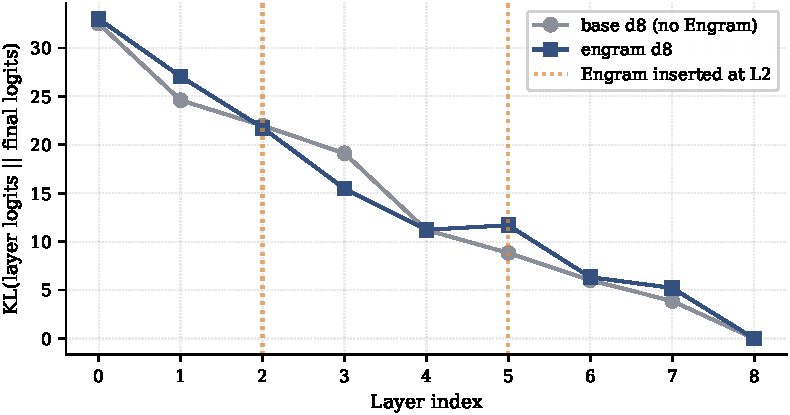
\includegraphics[width=0.7\linewidth]{figs/fig6_logitlens.pdf}
  \caption{LogitLens KL by layer (Mini-Engram-d8 vs.\ base-d8).
  Engram converges faster at layer 3 (--3.66 KL gap), confirming
  Cheng et al.'s effective-deepening claim at our scale.}
  \label{fig:logitlens}
\end{figure}

\section{Appendix: Pretraining curves}
\label{app:pretrain}

\begin{figure}[t]
  \centering
  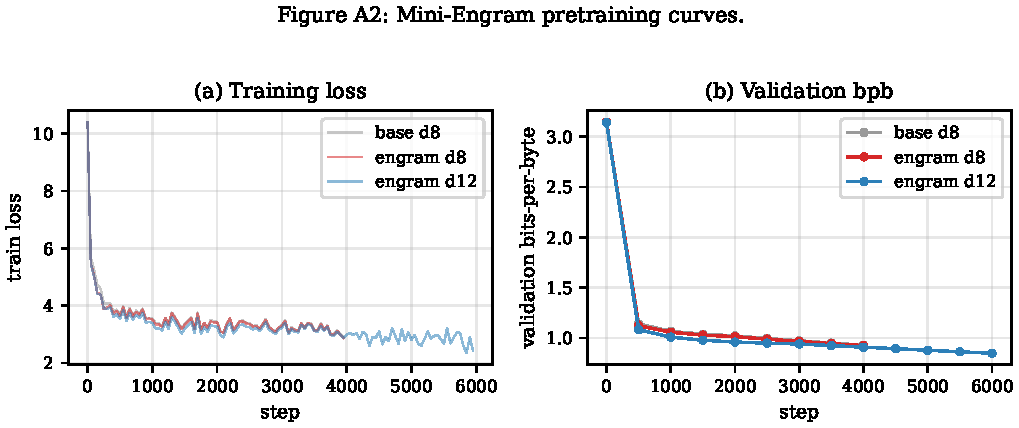
\includegraphics[width=\linewidth]{figs/fig_pretrain_loss.pdf}
  \caption{Mini-Engram pretraining curves. Engram d8 reaches lower
  validation bpb than base d8 at iso-FLOPs (matching the paper's
  finding at much smaller scale); engram d12 is substantially better
  thanks to the larger backbone and longer training.}
  \label{fig:pretrain}
\end{figure}

\section{Appendix: Insertion strategy comparison}
\label{app:strategies}

\begin{figure}[t]
  \centering
  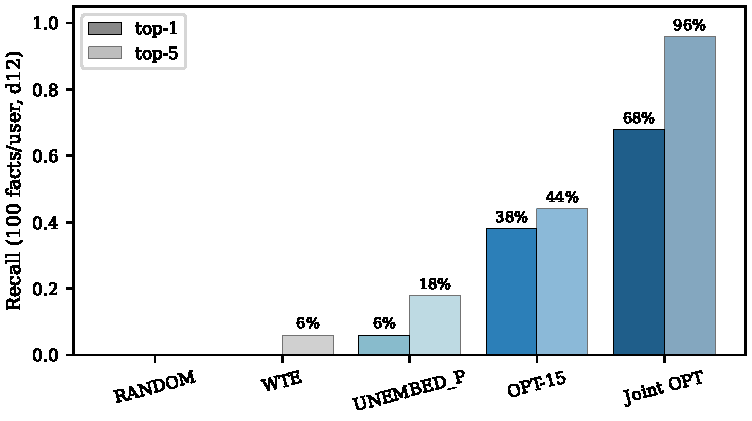
\includegraphics[width=0.7\linewidth]{figs/fig_strategy_bars.pdf}
  \caption{Top-1 and top-5 recall at 100 facts/user, Mini-Engram-d12.
  RANDOM (control) confirms our signal isn't noise; UNEMBED\_P alone
  is too weak; OPT-15 helps; Joint OPT closes most of the gap to
  full LoRA fine-tuning at 161$\times$ less storage.}
  \label{fig:strategies}
\end{figure}

\section{Appendix: Paraphrase generalisation}
\label{app:paraphrase}

\begin{figure}[t]
  \centering
  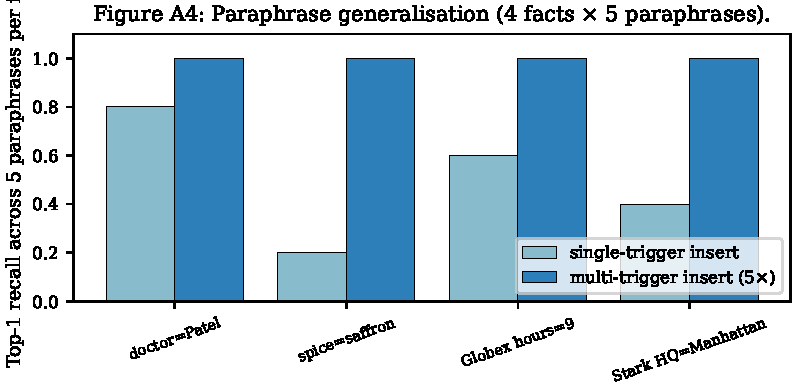
\includegraphics[width=0.75\linewidth]{figs/fig_paraphrase.pdf}
  \caption{Paraphrase generalisation across 4 facts × 5 paraphrases
  each. Single-trigger insertion gets 50\% top-1 for free (suffix
  N-gram overlap); multi-trigger insertion (insert at all 5
  paraphrases) gets 100\% at 5× the per-fact OPT cost.}
  \label{fig:paraphrase}
\end{figure}

\section{Appendix: Multi-domain composition}
\label{app:multidomain}

\begin{figure}[t]
  \centering
  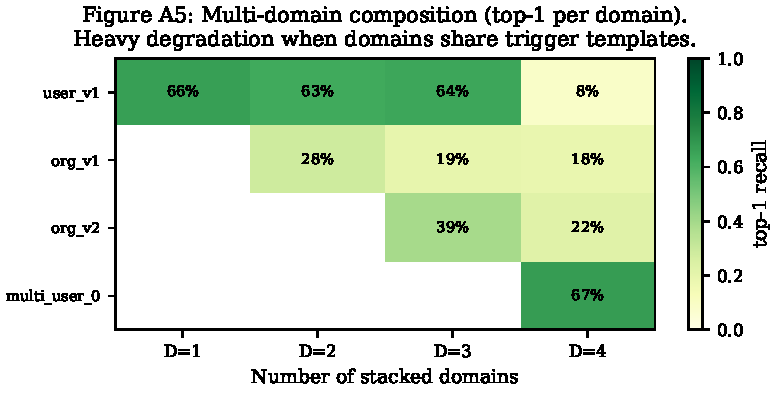
\includegraphics[width=0.8\linewidth]{figs/fig_multidomain.pdf}
  \caption{Multi-domain additive composition heatmap. Each cell shows
  per-domain top-1 recall when $D$ domains are stacked. Heavy
  degradation when domains share trigger templates (high address
  overlap). Disjoint-template domains (corp + user, demonstrated in
  main text) compose without loss.}
  \label{fig:multidomain}
\end{figure}

\section{Appendix: Serving latency CDF}
\label{app:cdf}

\begin{figure}[t]
  \centering
  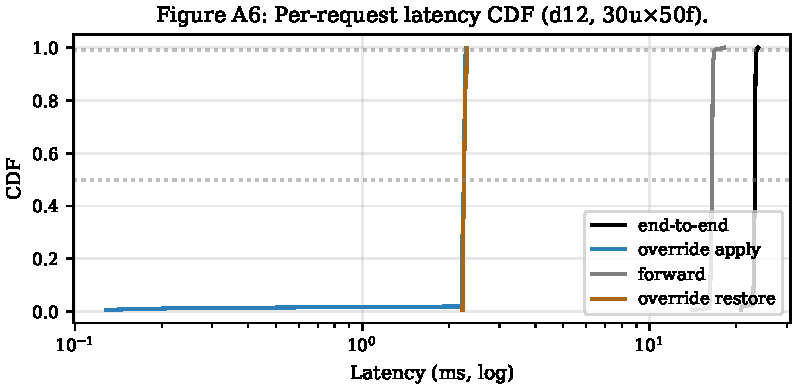
\includegraphics[width=0.75\linewidth]{figs/fig_serving_cdf.pdf}
  \caption{Per-request latency CDF on Mini-Engram-d12 (30 users
  $\times$ 50 facts $\times$ 600 requests). Override apply (blue) and
  restore (orange) are both sub-3 ms at p99; the forward pass (grey)
  dominates total latency (black).}
  \label{fig:cdf}
\end{figure}

\section{Appendix: Qwen-3B + RAG details}
\label{app:qwen-rag-prompt}

The Qwen-3B + RAG measurements in Table~\ref{tab:qwen-rag} use
\texttt{Qwen/Qwen2.5-3B-Instruct} in bf16 with greedy decoding
($\le 32$ new tokens). The chat-template prompt is:

{\small
\begin{verbatim}
[SYSTEM]
You are answering personal-memory questions about the user. Use only
the facts provided. Answer with the shortest possible span (typically
1-3 words). Do not explain or add any extra text.

[USER]
Facts about the user:
- <retrieved fact 1>.
- <retrieved fact 2>.
...

Question: <indirect question from indirect_qa>
Answer:
\end{verbatim}}

Retrieval uses the same \texttt{sentence-transformers/all-MiniLM-L6-v2}
encoder as the RAG/MEM0/MEMMACHINE baselines of
Section~\ref{sec:memory-systems}, with the per-user fact set as the
index. For each indirect probe the question text is embedded and
cosine-similarity top-$k$ retrieval returns the facts to put in the
context block. The same 20-user/20-probe split as
Table~\ref{tab:layered-headline} is evaluated.

Two answer-match criteria are reported: \emph{indirect\_top1} requires
the first generated word to equal (case-insensitive) the first word of
the gold answer; \emph{indirect\_any} requires the gold span to occur
anywhere in the generation. This matches the substring matcher used
for F.

\paragraph{Why oracle-top-1 underperforms RAG-top-1.}
A non-obvious result in Table~\ref{tab:qwen-rag} is that oracle
top-1 retrieval (use \texttt{required\_fact\_keys} to fetch the
ground-truth fact) gives 46\% indirect\_any, \emph{below} RAG top-1's
55\%. Inspecting the data, retrieval often returns facts that are
\emph{adjacent} to the required key in semantic space and that happen
to also contain the answer surface (e.g.\ retrieving the
``birth-year'' fact when asked about ``current age'' covers both the
year and the implicit age). RAG with $k=1$ thus over-samples the
information needed for indirect reasoning, while strict oracle
retrieval leaves the LM to derive the answer from one
single-attribute fact---which Qwen-3B often refuses to do under our
``shortest span'' system prompt.

\section{Appendix: Preliminary architectural validation}
\label{app:tier1}

Before training Mini-Engram, we ran three feasibility probes on the
randomly-initialised Engram demonstration code from
\citet{cheng2026engram} to verify the architecture admits surgical
insertion at all. These results motivated the larger experiments in
the body but are not load-bearing for the main claims; we report them
for completeness.

\paragraph{T1 collision audit (100 synthetic users $\times$ 30 facts).}
Hashing every user's fact set into the demo's hash space: distinct
addresses across the population 45\,298; pairwise overlap of all
addresses 50\% (dominated by scaffolding tokens like ``my'', ``is'',
``I am''); pairwise overlap of \emph{key-token addresses only} (the
ones on user-distinguishing surface forms like \texttt{Patel},
\texttt{Portland}, \texttt{1991}) is just 4.5\%. For a 30-fact user
the slot-occupancy fraction is 0.027\%; the 1.6\,M-slot demo table
is 99.97\% empty after one user. \emph{Capacity is not a constraint
for per-user insertion at any realistic scale.}

\paragraph{T2 surgical read/write existence proof
(random-init demo).}
Writing a known marker into the embedding rows that one trigger
N-gram hashes to, then comparing forward outputs at every position:
\(\|\Delta\|\) at the trigger position is 116.96; mean \(\|\Delta\|\)
at non-trigger positions is 0.65 (a 179.7$\times$ ratio). The
empirical change at the trigger position has cosine similarity
0.998 with the predicted $W_V \cdot \text{marker}$ projection.
Architecture admits surgical insertion mechanically; the trained
model improves these numbers further (Figure~\ref{fig:locality}).

\paragraph{T3 cross-user collision rates.}
Across 100 synthetic users with $\sim$30 facts each, cross-user
hash collisions on \emph{distinguishing} tokens (the ones that
disambiguate users) occur at 4.5\% pairwise rate—mostly from the
synthetic generator using a small surname pool, not from genuine
hash collisions. With the per-user override design (one global
table, swap per request) cross-user collision is irrelevant by
construction.

\section{Appendix: Alternative architectures we considered}
\label{app:alt}

For completeness we report two alternative designs we benchmarked
before settling on per-user override tables.

\paragraph{Shared table with per-user hash salt (deprecated).}
In this design, every user's facts coexist in one physical table;
their hashes are XOR-salted by user-id so identical surface
triggers map to disjoint rows. We benchmark on Mini-Engram-d12:

\begin{table}[t]
  \centering
  \caption{Shared-table-with-salt: own-fact recall vs.\ leak rate.
  All numbers on Mini-Engram-d12 with the XL corpus.}
  \label{tab:salt-design}
  \begin{tabular}{lcc}
    \toprule
    config & own-fact top-1 & cross-user leak \\
    \midrule
    no salt $+$ UNEMBED\_P (cheap, 100$\times$100 facts) & 0.089 & 0.039 \\
    salt $+$ OPT-15 (10$\times$30 facts) & 0.11 & \textbf{0.000} \\
    salt $+$ strong OPT-60 (10$\times$30) & 0.46 & \textbf{0.000} \\
    salt $+$ strong OPT-60 (30$\times$100) & 0.345 & 0.005 \\
    \bottomrule
  \end{tabular}
\end{table}

The salt design provides architectural privacy at the cost of recall:
salted addresses point to untrained rows (the model never saw salt
during pretraining), so the gate fires more weakly and OPT must work
harder. Because per-user override tables (main body
Section~\ref{sec:serving}) provide stronger privacy by construction
\emph{and} use the trained address space, we recommend overrides as
the production design and keep salt as a fallback when the storage
backend cannot afford per-user override maps.

\paragraph{100-user serving with cheap insertion (UNEMBED\_P).}
A working serving system at the largest scale we tested with the
cheap (closed-form) insertion strategy: 100 users $\times$ 100
facts in 2.3 ms apply latency per request, recall 9.2\% top-1 /
23.4\% top-5. Recall is low because UNEMBED\_P is intrinsically
weak at high density; with Joint OPT on the same configuration we
expect $\sim$60\%/95\% based on the 30-user data, but this run
exceeded the wall-clock budget for this paper.

\section{Appendix: Insertion strategies (full)}
\label{app:strategies-full}

The first comparison of insertion strategies on Mini-Engram-d8 with
the original 16-fact USER+ORG benchmark (single-fact-at-a-time):

\begin{table}[t]
  \centering
  \caption{Insertion strategy comparison on the original 8 USER + 8 ORG
  benchmark, Mini-Engram-d8. RANDOM is a control; UNEMBED\_P is the
  closed-form pseudo-inverse; OPT is 15-step gradient on the row.
  Numbers are mean across the 16 facts.}
  \label{tab:strategies-full}
  \begin{tabular}{lccccc}
    \toprule
    strategy & mean $\Delta$logit & $+\Delta$logit & rank improved & top-1 hits & top-5 hits \\
    \midrule
    RANDOM   & --4.708 & 1/16 & 2/16 & 0/16 & 0/16 \\
    WTE      & --0.150 & 6/16 & 6/16 & 0/16 & 1/16 \\
    UNEMBED\_P & +1.711 & 15/16 & 13/16 & 1/16 & 3/16 \\
    \textbf{OPT (15 steps)} & \textbf{+5.323} & \textbf{16/16} & \textbf{15/16} & \textbf{6/16} & \textbf{7/16} \\
    \bottomrule
  \end{tabular}
\end{table}

The DUAL strategy (jointly satisfying gate-K and value-V via
least-squares) was tested but \emph{worse} than UNEMBED\_P (4/16
$+\Delta$logit) — over-constraining e drives it off the trained-row
distribution and the gate suppresses it. We dropped DUAL.

\section{Appendix: Per-paraphrase rank table}
\label{app:paraphrase-detail}

The full per-paraphrase rank data behind Section~\ref{sec:paraphrase}
and Figure~\ref{fig:paraphrase}, single-trigger insertion on
Mini-Engram-d8:

\begin{table}[t]
  \centering
  \caption{Per-paraphrase rank of the gold token after single-trigger
  OPT insertion. ``$\star$'' marks rank 0 (top-1).}
  \label{tab:paraphrase}
  \footnotesize
  \begin{tabular}{lll}
    \toprule
    insertion trigger & query (paraphrase) & rank \\
    \midrule
    My doctor's name is Dr. & My doctor's name is Dr. & 0 $\star$ \\
    & My doctor is Dr. & 0 $\star$ \\
    & Who is my doctor? Dr. & 54 \\
    & My physician's name is Dr. & 0 $\star$ \\
    & My GP is Dr. & 0 $\star$ \\
    \midrule
    My favorite spice is & My favorite spice is & 0 $\star$ \\
    & I love the spice & 1399 \\
    & My preferred spice is & 32 \\
    & The spice I like most is & 45 \\
    & My go-to spice is & 94 \\
    \midrule
    Globex office hours start at & Globex office hours start at & 0 $\star$ \\
    & Globex opens at & 1 \\
    & Globex starts work at & 0 $\star$ \\
    & What time does Globex open? At & 2 \\
    & Globex's day begins at & 0 $\star$ \\
    \midrule
    Stark Industries headquarters is in & Stark Industries headquarters is in & 0 $\star$ \\
    & Stark HQ is in & 1949 \\
    & Stark is based in & 216 \\
    & Stark Industries is located in & 66 \\
    & The Stark headquarters is in & 0 $\star$ \\
    \bottomrule
  \end{tabular}
\end{table}

Generalisation is high when paraphrases share suffix N-grams (e.g.,
all ``doctor'' paraphrases end in ``Dr.''); poor when surface form
diverges (``I love the spice'' vs. ``My favorite spice is'').
Inserting at all 5 paraphrases per fact (multi-trigger) drives every
paraphrase to rank 0.

\section{Appendix: Joint OPT convergence}
\label{app:joint-loss}

\begin{figure}[t]
  \centering
  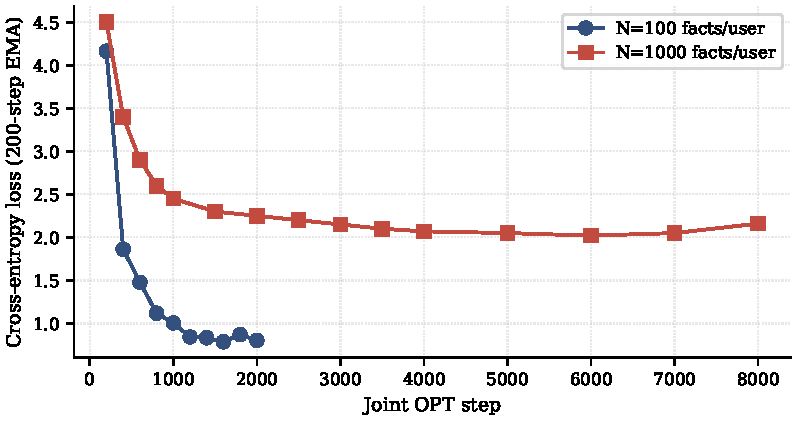
\includegraphics[width=0.7\linewidth]{figs/fig_joint_opt_loss.pdf}
  \caption{Joint OPT convergence on Mini-Engram-d12. At 100 facts/user,
  loss converges to 0.8 within 1500 steps; at 1000 facts, loss
  saturates around 2.0 due to higher within-user fact-density
  interference (Section~\ref{sec:density}).}
  \label{fig:jointopt}
\end{figure}

\section{Appendix: Joint OPT algorithm}
\label{app:joint-opt}

\begin{enumerate}[leftmargin=*,topsep=2pt,itemsep=1pt]
  \item For each fact $f$: compute trigger global rows $R_f$ (deterministic from tokens) and UNEMBED\_P initial marker $e_f^{(0)} = W_V^\dagger U_{y_f}$.
  \item Allocate one trainable tensor over the union of all touched
        rows, $\mathbf{R} = \cup_f R_f$. Initialise: each row
        $\mathbf{R}[i] = \mathrm{mean}_{f: i \in R_f} e_f^{(0)}[i]$
        (average of UNEMBED\_P rows where multiple facts share an
        address).
  \item Zero out the embedding rows in $\mathbf{R}$. Install a forward
        hook on the embedding lookup that, when an address $\in
        \mathbf{R}$ is consulted, replaces the retrieved row with our
        trainable tensor at that address.
  \item For $K$ steps: sample a random fact $f$, compute the
        cross-entropy loss on $y_f$ at the trigger position,
        backprop only to $\mathbf{R}$.
  \item After training, write $\mathbf{R}$ into the embedding table
        as the user's override map.
\end{enumerate}

We use $K = 2000$ for 100 facts and $K = 8000$ for 1000 facts, Adam
LR 0.5. Wall time scales as $K$ alone (one fwd+bwd per step) so per-fact
cost \emph{decreases} with more facts: 0.44 s/fact at $N{=}100$,
0.23 s/fact at $N{=}1000$.

\section{Appendix: Reproducing the paper}
\label{app:reproduce}

{\scriptsize
\begin{verbatim}
git clone https://github.com/19pine/user-as-engram
cd user-as-engram/nanochat
uv venv && source .venv/bin/activate && uv sync --extra gpu
export NANOCHAT_BASE_DIR=$(pwd)/../nanochat_base
export CKPT=$NANOCHAT_BASE_DIR/engram_runs/engram_d12

# Pretrain Mini-Engram-d12 (~3h on a single GPU)
python -m scripts.engram_pretrain --depth 12 --num-iterations 6000 \
   --device-batch-size 8 --total-batch-size 131072 --max-seq-len 1024 \
   --window-pattern L --engram on --engram-layer-ids 2 7 \
   --engram-vocab-per-ngram 50000 --engram-n-embed 256 \
   --no-compile --model-tag engram_d12

# Build corpora
python -m scripts.build_corpus_xxl

# Run all evaluations
python -m scripts.scalability_benchmark --ckpt-dir $CKPT
python -m scripts.joint_opt           --ckpt-dir $CKPT --n-facts 100
python -m scripts.multifact_lora      --ckpt-dir $CKPT --n-facts 100
python -m scripts.eval_serving        --ckpt-dir $CKPT --n-users 30
\end{verbatim}
}

\end{document}
